% Options for packages loaded elsewhere
\PassOptionsToPackage{unicode}{hyperref}
\PassOptionsToPackage{hyphens}{url}
%
\documentclass[
]{article}
\usepackage{lmodern}
\usepackage{amssymb,amsmath}
\usepackage{ifxetex,ifluatex}
\ifnum 0\ifxetex 1\fi\ifluatex 1\fi=0 % if pdftex
  \usepackage[T1]{fontenc}
  \usepackage[utf8]{inputenc}
  \usepackage{textcomp} % provide euro and other symbols
\else % if luatex or xetex
  \usepackage{unicode-math}
  \defaultfontfeatures{Scale=MatchLowercase}
  \defaultfontfeatures[\rmfamily]{Ligatures=TeX,Scale=1}
\fi
% Use upquote if available, for straight quotes in verbatim environments
\IfFileExists{upquote.sty}{\usepackage{upquote}}{}
\IfFileExists{microtype.sty}{% use microtype if available
  \usepackage[]{microtype}
  \UseMicrotypeSet[protrusion]{basicmath} % disable protrusion for tt fonts
}{}
\makeatletter
\@ifundefined{KOMAClassName}{% if non-KOMA class
  \IfFileExists{parskip.sty}{%
    \usepackage{parskip}
  }{% else
    \setlength{\parindent}{0pt}
    \setlength{\parskip}{6pt plus 2pt minus 1pt}}
}{% if KOMA class
  \KOMAoptions{parskip=half}}
\makeatother
\usepackage{xcolor}
\IfFileExists{xurl.sty}{\usepackage{xurl}}{} % add URL line breaks if available
\IfFileExists{bookmark.sty}{\usepackage{bookmark}}{\usepackage{hyperref}}
\hypersetup{
  hidelinks,
  pdfcreator={LaTeX via pandoc}}
\urlstyle{same} % disable monospaced font for URLs
\usepackage[margin=1in]{geometry}
\usepackage{graphicx}
\makeatletter
\def\maxwidth{\ifdim\Gin@nat@width>\linewidth\linewidth\else\Gin@nat@width\fi}
\def\maxheight{\ifdim\Gin@nat@height>\textheight\textheight\else\Gin@nat@height\fi}
\makeatother
% Scale images if necessary, so that they will not overflow the page
% margins by default, and it is still possible to overwrite the defaults
% using explicit options in \includegraphics[width, height, ...]{}
\setkeys{Gin}{width=\maxwidth,height=\maxheight,keepaspectratio}
% Set default figure placement to htbp
\makeatletter
\def\fps@figure{htbp}
\makeatother
\setlength{\emergencystretch}{3em} % prevent overfull lines
\providecommand{\tightlist}{%
  \setlength{\itemsep}{0pt}\setlength{\parskip}{0pt}}
\setcounter{secnumdepth}{-\maxdimen} % remove section numbering
\usepackage{float} \usepackage{caption} \captionsetup[table]{font=footnotesize} \captionsetup[figure]{font=footnotesize} \captionsetup[figure]{labelformat=empty} \captionsetup[table]{labelformat=empty} \usepackage{pdflscape} \newcommand{\blandscape}{\begin{landscape}} \newcommand{\elandscape}{\end{landscape}}
\usepackage{setspace}\onehalfspacing \usepackage{lineno}\linenumbers
\usepackage{booktabs}
\usepackage{longtable}
\usepackage{array}
\usepackage{multirow}
\usepackage{wrapfig}
\usepackage{float}
\usepackage{colortbl}
\usepackage{pdflscape}
\usepackage{tabu}
\usepackage{threeparttable}
\usepackage{threeparttablex}
\usepackage[normalem]{ulem}
\usepackage{makecell}
\usepackage{xcolor}
\ifluatex
  \usepackage{selnolig}  % disable illegal ligatures
\fi
\newlength{\cslhangindent}
\setlength{\cslhangindent}{1.5em}
\newenvironment{cslreferences}%
  {\setlength{\parindent}{0pt}%
  \everypar{\setlength{\hangindent}{\cslhangindent}}\ignorespaces}%
  {\par}

\author{}
\date{\vspace{-2.5em}}

\begin{document}

\raggedright

\textbf{Title:} Carbon cycling in mature and regrowth forests globally:
a macroecological synthesis based on the Global Forest Carbon (ForC)
database

\textbf{Authors:}

Kristina J. Anderson-Teixeira\textsuperscript{1,2}*

Valentine Herrmann\textsuperscript{1}

Becky Banbury Morgan\textsuperscript{1,3}

Ben Bond-Lamberty\textsuperscript{4}

Susan C. Cook-Patton\textsuperscript{5}

Abigail E. Ferson\textsuperscript{1,6}

Helene C. Muller-Landau\textsuperscript{2}

Maria M. H. Wang\textsuperscript{1,7}

\textbf{Author Affiliations:}

\begin{enumerate}
\def\labelenumi{\arabic{enumi}.}
\tightlist
\item
  Conservation Ecology Center; Smithsonian Conservation Biology
  Institute; National Zoological Park, Front Royal, VA 22630, USA
\item
  Center for Tropical Forest Science-Forest Global Earth Observatory;
  Smithsonian Tropical Research Institute; Panama, Republic of Panama
\item
  School of Geography, University of Leeds, Leeds, UK
\item
  Joint Global Change Research Institute, Pacific Northwest National
  Laboratory, College Park Maryland 20740, USA
\item
  The Nature Conservancy; Arlington VA 22203, USA
\item
  College of Natural Resources, University of Idaho; Moscow, Idaho
  83843, USA
\item
  Grantham Centre for Sustainable Futures and Department of Animal and
  Plant Sciences, University of Sheffield, Western Bank, Sheffield,
  South Yorkshire S10 2TN, UK
\end{enumerate}

*corresponding author:
\href{mailto:teixeirak@si.edu}{\nolinkurl{teixeirak@si.edu}}; +1 540 635
6546

\newpage

\hypertarget{summary}{%
\subsection{Summary}\label{summary}}

\emph{Background.} Earth's climate is closely linked to forests, which
strongly influence atmospheric carbon dioxide (CO\textsubscript{2}) and
climate by their impact on the global carbon (C) cycle. However, efforts
to incorporate forests into climate models and CO\textsubscript{2}
accounting frameworks have been constrained by a lack of accessible,
global-scale data on how C cycling varies across forest types and stand
ages.

\emph{Methods/Design.} Here, we draw from the Global Forest Carbon
Database, ForC, to provide a macroscopic overview of C cycling in the
world's forests, giving special attention to stand age-related
variation. Specifically, we use 11923 \emph{ForC} records from 865
geographic locations representing 34 C cycle variables to characterize
ensemble C budgets for four broad forest types (tropical broadleaf
evergreen, temperate broadleaf, temperate conifer, and taiga), including
estimates for both mature and regrowth (age \textless100 years) forests.
For regrowth forests, we quantify age trends for all variables with
sufficient data.

\emph{Review Results/ Synthesis.} \emph{ForC v3.0} yielded a
comprehensive picture of C cycling in the world's major forest biomes.
The rate of C cycling generally increased from boreal to tropical
regions in both mature and regrowth forests, whereas C stocks showed
less directional variation. The majority of flux variables, together
with most live biomass pools, increased significantly with stand age.
Importantly, there was generally good closure of C budgets, \emph{i.e.,}
internal consistency in the \emph{ForC} data.

\emph{Discussion.} As climate change accelerates, understanding and
managing the carbon dynamics of forests is critical to forecasting,
mitigation, and adaptation. This synthetic and internally consistent
global overview of C stocks and fluxes across biomes and stand ages will
help to advance these efforts.

\emph{Key words}: forest ecosystems; carbon cycle; stand age;
productivity; respiration; biomass; global

\newpage

\hypertarget{background}{%
\subsection{Background}\label{background}}

Forest ecosystems are shaping the course of climate change through their
influence on atmospheric carbon dioxide (CO\textsubscript{2}; Bonan
2008, Friedlingstein \emph{et al} 2019, IPCC 2018). Despite the
centrality of forest C cycling in regulating atmospheric
CO\textsubscript{2}, important uncertainties in climate models
(Friedlingstein \emph{et al} 2006, Krause \emph{et al} 2018, Bonan
\emph{et al} 2019, Di Vittorio \emph{et al} 2020) and
CO\textsubscript{2} accounting frameworks (Pan \emph{et al} 2011) can be
traced to lack of accessible, comprehensive data on how C cycling varies
across forest types and in relation to stand history. These require
large-scale databases with global coverage, which runs contrary to the
nature in which forest C stocks and fluxes are measured and published.
While remote sensing measurements are increasingly useful for global- or
regional-scale estimates of a few critical variables (e.g., aboveground
biomass: Hu \emph{et al} 2016, Spawn \emph{et al} 2020, gross primary
productivity, \(GPP\): Li and Xiao 2019, Saatchi \emph{et al} 2011),
measurement and validation of most forest C stocks and fluxes require
intensive on-the-ground data collection.

A robust understanding of forest impacts on global C cycling is
essential. Annual gross CO\textsubscript{2} sequestration in forests
(gross primary productivity, \(GPP\)) is estimated at \textgreater69 Gt
C yr\textsuperscript{-1} (Badgley \emph{et al} 2019), or \textgreater7
times average annual fossil fuel emissions from 2009-2018 (9.5 \(\pm\)
0.5 Gt C yr\textsuperscript{-1}; Friedlingstein \emph{et al} 2019). Most
of this enormous C sequestration is counterbalanced by
CO\textsubscript{2} releases to the atmosphere through ecosystem
respiration (\(R_{eco}\)) or fire, with forests globally dominant as
sources of both soil respiration (Warner \emph{et al} 2019) and fire
emissions (Werf \emph{et al} 2017). In recent years, the remaining
CO\textsubscript{2} sink averaged 3.2 \(\pm\) 0.6 GtC
yr\textsuperscript{-1} from 2009-2018, offsetting 29\% of anthropogenic
fossil fuel emissions (Friedlingstein \emph{et al} 2019). Yet, this sink
is reduced by deforestation, estimated at \textasciitilde1 Gt C
yr\textsuperscript{-1} in recent decades (Pan \emph{et al} 2011,
Tubiello \emph{et al} 2020), reducing the net forest sink to
\textasciitilde1.1-2.2 Gt C yr\textsuperscript{-1} across Earth's
forests (Friedlingstein \emph{et al} 2019).

The future of the current forest C sink is dependent both upon forest
responses to climate change itself and human land use decisions, which
will feedback and strongly influence the course of climate change.
Regrowing forests in particular will play an important role (Pugh
\emph{et al} 2019), as almost two-thirds of the world's forests were
secondary as of 2010 (FAO 2010). As anthropogenic and climate-driven
disturbances impact an growing proportion of Earth's forests (Andela
\emph{et al} 2017, McDowell \emph{et al} 2020), understanding the carbon
dynamics of regrowth forests is increasingly important
(Anderson‐Teixeira \emph{et al} 2013). Although age trends in
aboveground biomass have been relatively well-studied and synthesized
globally (Cook-Patton \emph{et al} 2020), a relative dearth of data and
synthesis on other C stocks and fluxes in secondary forests points to an
under-filled need to characterize age-related trends in forest C
cycling. Such understanding is particularly critical for reducing
uncertainty regarding the potential for carbon uptake and climate change
mitigation by regrowth forests (Krause \emph{et al} 2018, Cook-Patton
\emph{et al} 2020). Understanding, modeling, and managing
forest-atmosphere CO\textsubscript{2} exchange is thus central to
efforts to mitigate climate change (Grassi \emph{et al} 2017, Griscom
\emph{et al} 2017, Cavaleri \emph{et al} 2015).

Despite the importance of forests, comprehensive global studies have
historically been limited by the scattered and more local nature of
research studies. Primary research articles typically cover only a small
numbers of sites at a time. The rare exceptions that span regions or
continents with rare exceptions spanning regions or continents are
typically coordinated through research networks such as ForestGEO
(Anderson-Teixeira \emph{et al} 2015, e.g., Lutz \emph{et al} 2018),
NEON (Schimel \emph{et al} 2007), or FLUXNET (Baldocchi \emph{et al}
2001, e.g., Novick \emph{et al} 2018). The result of decades of research
on forest C cycling is that tens of thousands of records have been
distributed across literally thousands of scientific articles --often
behind paywalls-- along with variation in data formats, units,
measurement methods, \emph{etc.} In this format, the data are
effectively inaccessible for many global-scale analyses, including those
attempting to benchmark model performance with global data (Clark et al
2017, Luo et al 2012), quantify the the role of forests in the global C
cycle (\emph{e.g.}, Pan \emph{et al} 2011), or use book-keeping methods
to quantify actual or scenario-based exchanges of CO\textsubscript{2}
between forests and the atmosphere (Griscom \emph{et al} 2017, Houghton
2020).

To address the need for global-scale analyses of forest C cycling, we
recently developed \emph{ForC} (Anderson-Teixeira \emph{et al} 2016,
2018). \emph{ForC} contains published estimates of forest ecosystem C
stocks and annual fluxes (\textgreater50 variables), with the different
variables capturing the unique ecosystem pools (e.g., woody, foliage,
and root biomass; dead wood) and flux types (e.g, gross and net primary
productivity; soil, root, and ecosystem respiration). These data are
ground-based measurements, and \emph{ForC} contains associated data
required for interpretation (\emph{e.g.}, stand history, measurement
methods). Data have been amalgamated from original peer-reviewed
publications, either directly or via intermediary data compilations.
Since the its most recent publication (Anderson-Teixeira \emph{et al}
2018), \emph{ForC} has grown to include two additional large databases:
the Global Soil Respiration Database (SRDB; Bond-Lamberty and Thomson
2010) and the Global Reforestation Opportunity Assessment database
(GROA; Cook-Patton \emph{et al} 2020) that also synthesized published
forest C data. Following these additions, \emph{ForC} currently contains
39762 records from 10608 plots and 1532 distinct geographic areas
representing all forested biogeographic and climate zones. This
represents an 129\% increase in records from the prior publication
(Anderson-Teixeira \emph{et al} 2018).

Here, we provide a robust and comprehensive analysis of carbon cycling
from a stand to global level, and by biome and stand age, using the
largest global compilation of forest carbon data, which is available in
our open source Global Carbon Forest database (\emph{ForC}; Fig. 1). Our
primary goal is to provide a data-driven summary of our current state of
knowledge on broad trends in forest C cycling. Specifically, we address
three broad questions:

\begin{enumerate}
\def\labelenumi{\arabic{enumi}.}
\item
  How thoroughly can we represent C budgets for each of the world's
  major forest biomes (\emph{i.e.}, tropical, temperate broadleaf and
  deciduous, boreal) based on the current \emph{ForC} data?
\item
  How do C cycling vary across the world's major forest biomes?
\item
  How does C cycling vary with stand age (in interaction with biome)?
\end{enumerate}

While components of these questions have been previously addressed
(Luyssaert \emph{et al} 2007, Anderson-Teixeira \emph{et al} 2016,
Cook-Patton \emph{et al} 2020, Banbury Morgan \emph{et al} n.d.), our
analysis represents by far the most comprehensive analysis of C cycling
in global forests, and will serve as a foundation for improved
understanding of global forest C cycling and highlight where key sources
of uncertainty still reside.

\begin{figure}[H]

{\centering \includegraphics[width=1\linewidth]{tables_figures/World_Map_records_in_Biomes} 

}

\caption{Figure 1 | Map of sites included in this analysis. Symbols are colored according to the number of records at each site. Underlying map shows coverage of evergreen, deciduous, and mixed forests (from SYNMAP; Jung et al. 2006) and biomes. Distribution of sites, plots, and records among biomes is shown in the inset.}\label{fig:unnamed-chunk-5}
\end{figure}

\hypertarget{methods-design}{%
\subsection{Methods/ Design}\label{methods-design}}

This review synthesizes data from the \emph{ForC} database (Fig. 1;
\url{https://github.com/forc-db/ForC}; Anderson-Teixeira \emph{et al}
2016, 2018). \emph{ForC} amalgamates numerous intermediary data sets
(\emph{e.g.}, Luyssaert \emph{et al} 2007, Bond-Lamberty and Thomson
2010, Cook-Patton \emph{et al} 2020) and original studies. Original
publications were referenced to check values and obtain information not
contained in intermediary data sets, although this process has not been
completed for all records. The database was developed with goals of
understanding how C cycling in forests varies across broad geographic
scales and as a function of stand age. As such, there has been a focus
on incorporating data from regrowth forests (\emph{e.g.}, Anderson et al
2006, Martin et al 2013, Bonner et al 2013) and obtaining stand age data
when possible (83\% of records in v.2.0; Anderson-Teixeira \emph{et al}
2018). Particular attention was given to developing the database for
tropical forests (Anderson-Teixeira \emph{et al} 2016), which
represented roughly one-third of records in \emph{ForC} v2.0
(Anderson-Teixeira \emph{et al} 2018). Since publication of ForC v2.0,
we added the following data to ForC: the Global Database of Soil
Respiration Database (\emph{SRDB} v4, 9488 records; Bond-Lamberty and
Thomson 2010), the Global Reforestation Opportunity Assessment database
(\emph{GROA} v1.0, 10116 records; Cook-Patton \emph{et al} 2020,
Anderson-Teixeira \emph{et al} 2020). We have also added data from
individual publications, with a particular focus on productivity (e.g.,
Taylor \emph{et al} 2017), dead wood, and ForestGEO sites (e.g., Lutz
\emph{et al} 2018, p @johnson\_climate\_2018). The database version used
for this analysis has been tagged as a new release on Github (v3.0) and
assigned a DOI through Zenodo (DOI: TBD).

To facilitate analyses, we created a simplified version of ForC,
\emph{ForC-simplified}
(\url{https://github.com/forc-db/ForC/blob/master/ForC_simplified}),
which we analyzed here. In generating \emph{ForC-simplified}, all
measurements originally expressed in units of dry organic matter
(\(OM\)) were converted to units of C using the IPCC default of
\(C = 0.47 * OM\) (IPCC 2018). Duplicate or otherwise conflicting
records were reconciled as described in Appendix S1, resulting in a
total of 22265 records (56\% size of total database). Records were
filtered to remove plots that had undergone significant anthropogenic
management or major disturbance since the most recent stand initiation
event. Specifically, we removed all plots flagged as managed in
ForC-simplified (13.9\%). This included plots with any record of
managements manipulating CO\textsubscript{2}, temperature, hydrology,
nutrients, or biota, as well as any plots whose site or plot name
contained the terms ``plantation'', ``planted'', ``managed'',
``irrigated'', or ``fertilized''. Plots flagged as disturbed in
ForC-simplified (5.6\%) included stands that had undergone any notable
anthropogenic thinning or partial harvest. We retained sites that were
grazed or had undergone low severity natural disturbances (\textless10\%
mortality) including droughts, major storms, fires, and floods. We
removed all plots for which no stand history information had been
retrieved (5.7\%). In total, this resulted in 17349 records (43.6\% of
the records in the database) being eligible for inclusion in the
analysis.

We selected 23 annual flux and 11 C stock variables for inclusion in the
analysis (Table 1). These different flux and stock variables represent
different pools (e.g., aboveground biomass, root biomass, dead wood) and
levels of combination (e.g., total net primary productivity, \(NPP\),
versus the individual elements of \(NPP\) such as foliage, roots, and
branches). Note that two flux variables, aboveground heterotropic
(\(R_{het-ag}\)) and total (\(R_{het}\)) respiration, were included for
conceptual completeness but had no records in \emph{ForC} (Table 1).
Records for our focal variables represented 90.3\% of the total records
eligible for inclusion. For this analysis, we combined some of ForC's
specific variables into more broadly defined variables. Specifically,
net ecosystem exchange (measured by eddy-covariance; Baldocchi \emph{et
al} 2001) and biometric estimates of \(NEP\) were combined into the
single variable \(NEP\) (Table 1). Furthermore, for \(NPP\), aboveground
\(NPP\) (\(ANPP\)), and the litterfall component of \(ANPP\)
(\(ANPP_{litterfall}\)), \emph{ForC} variables specifying inclusion of
different components were combined (\emph{e.g.}, measurements including
or excluding fruit and flower production and herbivory). Throughout
ForC, for all measurements drawing from tree census data (\emph{e.g.},
biomass, productivity), the minimum diameter breast height (DBH)
threshold for tree census was \(\le\) 10cm. All records were measured
directly or derived from field measurements (as opposed to modeled).

\begin{table}[!h]

\caption{\label{tab:unnamed-chunk-7}Table 1. Carbon cycle variables included in this analysis, their sample sizes, and summary of biome differences and age trends.}
\centering
\resizebox{\linewidth}{!}{
\fontsize{12}{14}\selectfont
\begin{tabular}[t]{l>{\raggedright\arraybackslash}p{7cm}>{\raggedleft\arraybackslash}p{1.1cm}>{\raggedleft\arraybackslash}p{1cm}>{\raggedleft\arraybackslash}p{1.8cm}ll}
\toprule
\multicolumn{1}{c}{ } & \multicolumn{1}{c}{ } & \multicolumn{3}{c}{N records} & \multicolumn{1}{c}{ } & \multicolumn{1}{c}{ } \\
\cmidrule(l{3pt}r{3pt}){3-5}
Variable & Description & records & plots & geographic areas & biome differences\textsuperscript{*} & age trend\textsuperscript{\dag}\\
\midrule
\addlinespace[0.3em]
\multicolumn{2}{l}{\textbf{Annual fluxes}}\\
\hspace{1em}$NEP$ & net ecosystem production or net ecosystem exchange (+ indicates C sink) & 329 & 146 & 88 & n.s. & +; xB\\
\hspace{1em}$GPP$ & gross primary production ($NPP + R_{auto}$ or $R_{eco}-NEE$) & 303 & 115 & 84 & TrB > TeB $\ge$ TeN $\ge$ BoN & +; xB\\
\hspace{1em}$NPP$ & net primary production ($ANPP$ + $BNPP$) & 214 & 112 & 74 & TrB > TeB $\ge$ TeN > BoN & n.s.\\
\hspace{1em}$ANPP$ & aboveground $NPP$ & 343 & 236 & 131 & TrB > TeB $\ge$ TeN > BoN & +; xB\\
\hspace{1em}$ANPP_{woody}$ & woody production ($ANPP_{stem}$ + $ANPP_{branch}$) & 64 & 53 & 37 & n.s. & +\\
\hspace{1em}$ANPP_{stem}$ & woody stem production & 217 & 190 & 117 & TrB > TeN $\ge$ TeB $\ge$ BoN & n.s.\\
\hspace{1em}$ANPP_{branch}$ & branch turnover & 69 & 59 & 42 & TrB > TeB $\ge$ TeN & n.s.\\
\hspace{1em}$ANPP_{foliage}$ & foliage production, typically estimated as annual leaf litterfall & 162 & 132 & 88 & TrB > TeB $\ge$ TeN > BoN & +\\
\hspace{1em}$ANPP_{litterfall}$ & litterfall, including leaves, reproductive structures, twigs, and sometimes branches & 82 & 70 & 55 & n.s. & +\\
\hspace{1em}$ANPP_{repro}$ & production of reproductive structures (flowers, fruits, seeds) & 51 & 44 & 34 & n.t. & n.t.\\
\hspace{1em}$ANPP_{folivory}$ & foliar biomass consumed by folivores & 20 & 12 & 11 & n.t. & n.t.\\
\hspace{1em}$M_{woody}$ & woody mortality--i.e., $B_{ag}$ of trees that die & 18 & 18 & 18 & n.t. & n.t.\\
\hspace{1em}$BNPP$ & belowground NPP ($BNPP_{coarse}$+ $BNPP_{fine}$) & 148 & 116 & 79 & TrB > TeN $\ge$ TeB $\ge$ BoN & +\\
\hspace{1em}$BNPP_{coarse}$ & coarse root production & 77 & 56 & 36 & TeN $\ge$ TrB & n.s.\\
\hspace{1em}$BNPP_{fine}$ & fine root production & 123 & 99 & 66 & n.s. & +\\
\hspace{1em}$R_{eco}$ & ecosystem respiration ($R_{auto}$+ $R_{het}$) & 213 & 98 & 70 & TrB > TeB $\ge$ TeN & +\\
\hspace{1em}$R_{auto}$ & autotrophic respiration ($R_{auto-ag}+ R_{root}$) & 24 & 23 & 15 & n.t. & n.t.\\
\hspace{1em}$R_{auto-ag}$ & aboveground autotrophic respiration (i.e., leaves and stems) & 2 & 2 & 1 & n.t. & n.t.\\
\hspace{1em}$R_{root}$ & root respiration & 181 & 139 & 95 & TrB $\ge$ TeB & +\\
\hspace{1em}$R_{soil}$ & soil respiration ($R_{het-soil} + R_{root}$) & 627 & 411 & 229 & TrB > TeB > TeN $\ge$ BoN & n.s.\\
\hspace{1em}$R_{het-soil}$ & soil heterotrophic respiration & 197 & 156 & 100 & TrB > TeB $\ge$ TeN & n.s.\\
\hspace{1em}$R_{het-ag}$ & aboveground heterotrophic respiration & 0 & 0 & 0 & - & -\\
\hspace{1em}$R_{het}$ & heterotrophic respiration ($R_{het-ag} +R_{het-soil}$) & 0 & 0 & 0 & - & -\\
\addlinespace[0.3em]
\multicolumn{2}{l}{\textbf{Stocks}}\\
\hspace{1em}$B_{tot}$ & total live biomass ($B_{ag}$+$B_{root}$) & 188 & 157 & 87 & TrB $\ge$ TeB > BoN & +; xB\\
\hspace{1em}$B_{ag}$ & aboveground live biomass  ($B_{ag-wood}$+$B_{foliage}$) & 4466 & 4072 & 621 & TrB $\ge$ TeN $\ge$ TeB > BoN & +; xB\\
\hspace{1em}$B_{ag-wood}$ & woody component of aboveground biomass & 115 & 102 & 64 & TeN > TrB $\ge$ BoN & +; xB\\
\hspace{1em}$B_{foliage}$ & foliage biomass & 134 & 115 & 72 & TeN > TrB $\ge$ BoN $\ge$ TeB & +; xB\\
\hspace{1em}$B_{root}$ & total root biomass ($B_{root-coarse}$+$B_{root-fine}$) & 2329 & 2298 & 360 & n.s. & +; xB\\
\hspace{1em}$B_{root-coarse}$ & coarse root biomass & 134 & 120 & 73 & TeN > TeB $\ge$ BoN & +; xB\\
\hspace{1em}$B_{root-fine}$ & fine root biomass & 226 & 180 & 109 & n.s. & +; xB\\
\hspace{1em}$DW_{tot}$ & deadwood ($DW_{standing}$+$DW_{down}$) & 79 & 73 & 42 & n.t. & +; xB\\
\hspace{1em}$DW_{standing}$ & standing dead wood & 36 & 35 & 22 & n.t. & n.t.\\
\hspace{1em}$DW_{down}$ & fallen dead wood, including coarse and sometimes fine woody debris & 278 & 265 & 37 & n.t. & +; xB\\
\hspace{1em}$OL$ & organic layer $/$ litter$/$ forest floor & 474 & 413 & 115 & n.s. & +; xB\\
\bottomrule
\multicolumn{7}{l}{\rule{0pt}{1em}\textsuperscript{*} Tr: Tropical, TeB: Temperate Broadleaf, TeN: Temperate Needleleaf, B: Boreal, n.s.: no significant differences, n.t.: not tested }\\
\multicolumn{7}{l}{\rule{0pt}{1em}\textsuperscript{\dag} + or -: significant positive or negative trend, xB: significant age x biome interaction, n.s.: no significant age trend, n.t.: not tested}\\
\end{tabular}}
\end{table}

We grouped forests into four broad biome types based on climate zones
and dominant vegetation type (tropical broadleaf, temperate broadleaf,
temperate needleleaf, and boreal needleleaf) and two age classifications
(young and mature). Climate zones (Fig. 1) were defined based on site
geographic coordinates according to Köppen-Geiger zones (Rubel and
Kottek 2010). We defined the tropical biome as including all equatorial
(A) zones, temperate biomes as including all warm temperate (C) zones
and warmer snow climates (Dsa, Dsb, Dwa, Dwb, Dfa, and Dfb), and the
boreal biome as including the colder snow climates (Dsc, Dsd, Dwc, Dwd,
Dfc, and Dfd). Any forests in dry (B) and polar (E) Köppen-Geiger zones
were excluded from the analysis. We defined leaf type (broadleaf /
needleleaf) was based on descriptions in original publications
(prioritized) or values extracted from a global map based on satellite
observations (SYNMAP; Jung \emph{et al} 2006). For young tropical
forests imported from \emph{GROA} but not yet classified by leaf type,
we assumed that all were broadleaf, consistent with the rarity of
naturally regenerating needleleaf forests in the tropics. We also
classified forests as ``young'' (\textless{} 100 years) or ``mature''
(\(\ge\) 100 years or classified as ``mature'', ``old growth'',
``intact'', or ``undisturbed'' in original publication). Assigning
stands to these groupings required the exclusion of records for which
\emph{ForC} lacked geographic coordinates (0.4\% of sites in full
database) or records of stand age (5.7\% of records in full database).
We also excluded records of stand age = 0 year (0.8\% of records in full
database). In total, our analysis retained 76.1 of the focal variable
records for forests of known age. Numbers of records by biome and age
class are given in Table S1.

Data were summarized to produce schematics of C cycling across the eight
biome by age group combinations identified above. To obtain the values
reported in the C cycle schematics, we first averaged any repeated
measurements within a plot. Values were then averaged across
geographically distinct areas, defined as plots clustered within 25 km
of one another (\emph{sensu} Anderson-Teixeira \emph{et al} 2018),
weighting by area sampled if available for all records. This step was
taken to avoid pseudo-replication.

We tested whether the C budgets described above ``closed''--\emph{i.e.},
whether they were internally consistent. Specifically, we first defined
relationships among variables: for example, \(NEP = GPP - R_{eco}\),
\(BNPP = BNPP_{coarse} + BNPP_{fine}\),
\(DW_{tot} = DW_{standing} + DW_{down}\)). Henceforth, we refer to the
variables on the left side of the equation as ``aggregate'' fluxes or
stocks, and those that are summed as ``component'' fluxes or stocks,
noting that the same variable can take both aggregate and component
positions in different relationships. We considered the C budget for a
given relationship ``closed'' when component variables summed to within
one standard deviation of the aggregate variable.

To test for differences across mature forest biomes, we also examined
how stand age impacted fluxes and stocks, employing a mixed effects
model (``lmer'' function in ``lme4'' R package; Bates \emph{et al} 2015)
with biome as fixed effect and plot nested within geographic.area as
random effects on the intercept. When Biome had a significant effect, we
looked at a Tukey's pairwise comparison to see which biomes were
significantly different from one another. This analysis was run for
variables with records for at least seven distinct geographic areas in
more than one biome, excluding any biomes that failed this criteria
(Table 1).

To test for age trends in young (\textless100yrs) forests, we employed a
mixed effects model with biome and log10{[}stand.age{]} as fixed effects
and plot nested within geographic.area as a random effect on the
intercept. This analysis was run for variables with records for at least
three distinct geographic areas in more than one biome, excluding any
biomes that failed this criteria (Table 1). When the effect of stand age
was significant at p \(\le\) 0.05 and when each biome had records for
stands of at least 10 different ages, a biome \(\times\) stand.age
interaction was included in the model.

To facilitate the accessibility of our results and data, and to allow
for rapid updates as additional data become available, we have automated
all database manipulation, analyses, and figure production in R (R Core
Team 2020).

\hypertarget{review-results-synthesis}{%
\subsection{Review Results/ Synthesis}\label{review-results-synthesis}}

\hypertarget{data-coverage}{%
\subsubsection{Data Coverage}\label{data-coverage}}

Of the 39762 records in \emph{ForC} v3.0, 11923 met our strict criteria
for inclusion in this study (Fig. 1). These records were distributed
across 5062 plots in 865 distinct geographic areas. Of the 23 flux and
11 stock variables mapped in these diagrams, \emph{ForC} contained
sufficient mature forest data for inclusion in our statistical analyses
(\emph{i.e.}, records from \(\ge\) 7 distinct geographic areas) for 20
fluxes and 9 stocks in tropical broadleaf forests, 15 fluxes and 8
stocks in temperate broadleaf forests, 14 fluxes and 7 stocks in
temperate conifer forests, and 8 fluxes and 7 stocks in boreal forests.
For regrowth forests (\textless100 yrs), \emph{ForC} contained
sufficient data for inclusion in our statistical analyses (\emph{i.e.},
records from \(\ge\) 3 distinct geographic areas) for 11 fluxes and 10
stocks in tropical broadleaf forests, 16 fluxes and 10 stocks in
temperate broadleaf forests, 16 fluxes and 10 stocks in temperate
conifer forests, and 14 fluxes and 9 stocks in boreal forests.

\hypertarget{c-cycling-in-mature-forests}{%
\subsubsection{C cycling in mature
forests}\label{c-cycling-in-mature-forests}}

Average C cycles for mature tropical broadleaf, temperate broadleaf,
temperate conifer, and boreal forests \(\ge\) 100 years old and with no
known major natural or anthropogenic disturbance are presented in
Figures 2-5 (and available in tabular format in the \emph{ForC} release
accompanying this publication:
\texttt{ForC/numbers\_and\_facts/ForC\_variable\_averages\_per\_Biome.csv}).

For variables with records from \(\ge\) 7 distinct geographic areas,
these ensemble C budgets were generally consistent. That is, component
variables summed to within one standard deviation of their respective
aggregate variables in all but one instance. In the temperate conifer
biome, the average composite measure of root biomass (\(B_{root}\)) was
less than the combined average value of coarse and fine root biomass
(\(B_{root-coarse}\) and \(B_{root-fine}\), respectively). This lack of
closure was driven by very high estimates of \(B_{root-coarse}\) from
high-biomass forests of the US Pacific Northwest.

\begin{landscape}
\begin{figure}[H]

{\centering \includegraphics[width=1\linewidth]{/Users/kteixeira/Dropbox (Smithsonian)/GitHub/ForC-db/ForC/figures/C_cycle_diagrams/Diagrams/Tropical broadleaf MATURE} 

}

\caption{Figure 2 | C cycle diagram for mature tropical broadleaf forests. Arrows indicate fluxes (Mg C ha$^{-1}$ yr$^{-1}$); boxes indicate stocks (Mg C ha$^{-1}$), with variables as defined in Table 1. Presented are mean ± std, where geographically distinct areas are treated as the unit of replication. Dashed shape outlines indicate variables with records from <7 distinct geographic areas, and dashed arrows indicate fluxes with no data. To illustrate the magnitude of different fluxes, arrow size is proportional to the square root of corresponding flux. Asterisk after variable name indicates lack of C cycle closure.}\label{fig:unnamed-chunk-9}
\end{figure}

\begin{figure}[H]

{\centering \includegraphics[width=1\linewidth]{/Users/kteixeira/Dropbox (Smithsonian)/GitHub/ForC-db/ForC/figures/C_cycle_diagrams/Diagrams/Temperate broadleaf MATURE} 

}

\caption{Figure 3 | C cycle diagram for mature temperate broadleaf forests. Arrows indicate fluxes (Mg C ha$^{-1}$ yr$^{-1}$); boxes indicate stocks (Mg C ha$^{-1}$), with variables as defined in Table 1. Presented are mean ± std, where geographically distinct areas are treated as the unit of replication. Dashed shape outlines indicate variables with records from <7 distinct geographic areas, and dashed arrows indicate fluxes with no data. To illustrate the magnitude of different fluxes, arrow size is proportional to the square root of corresponding flux. Asterisk after variable name indicates lack of C cycle closure.}\label{fig:unnamed-chunk-10}
\end{figure}

\begin{figure}[H]

{\centering \includegraphics[width=1\linewidth]{/Users/kteixeira/Dropbox (Smithsonian)/GitHub/ForC-db/ForC/figures/C_cycle_diagrams/Diagrams/Temperate conifer MATURE} 

}

\caption{Figure 4 | C cycle diagram for mature temperate conifer forests. Arrows indicate fluxes (Mg C ha$^{-1}$ yr$^{-1}$); boxes indicate stocks (Mg C ha$^{-1}$), with variables as defined in Table 1. Presented are mean ± std, where geographically distinct areas are treated as the unit of replication. Dashed shape outlines indicate variables with records from <7 distinct geographic areas, and dashed arrows indicate fluxes with no data. To illustrate the magnitude of different fluxes, arrow size is proportional to the square root of corresponding flux. Asterisk after variable name indicates lack of C cycle closure.}\label{fig:unnamed-chunk-11}
\end{figure}

\begin{figure}[H]

{\centering 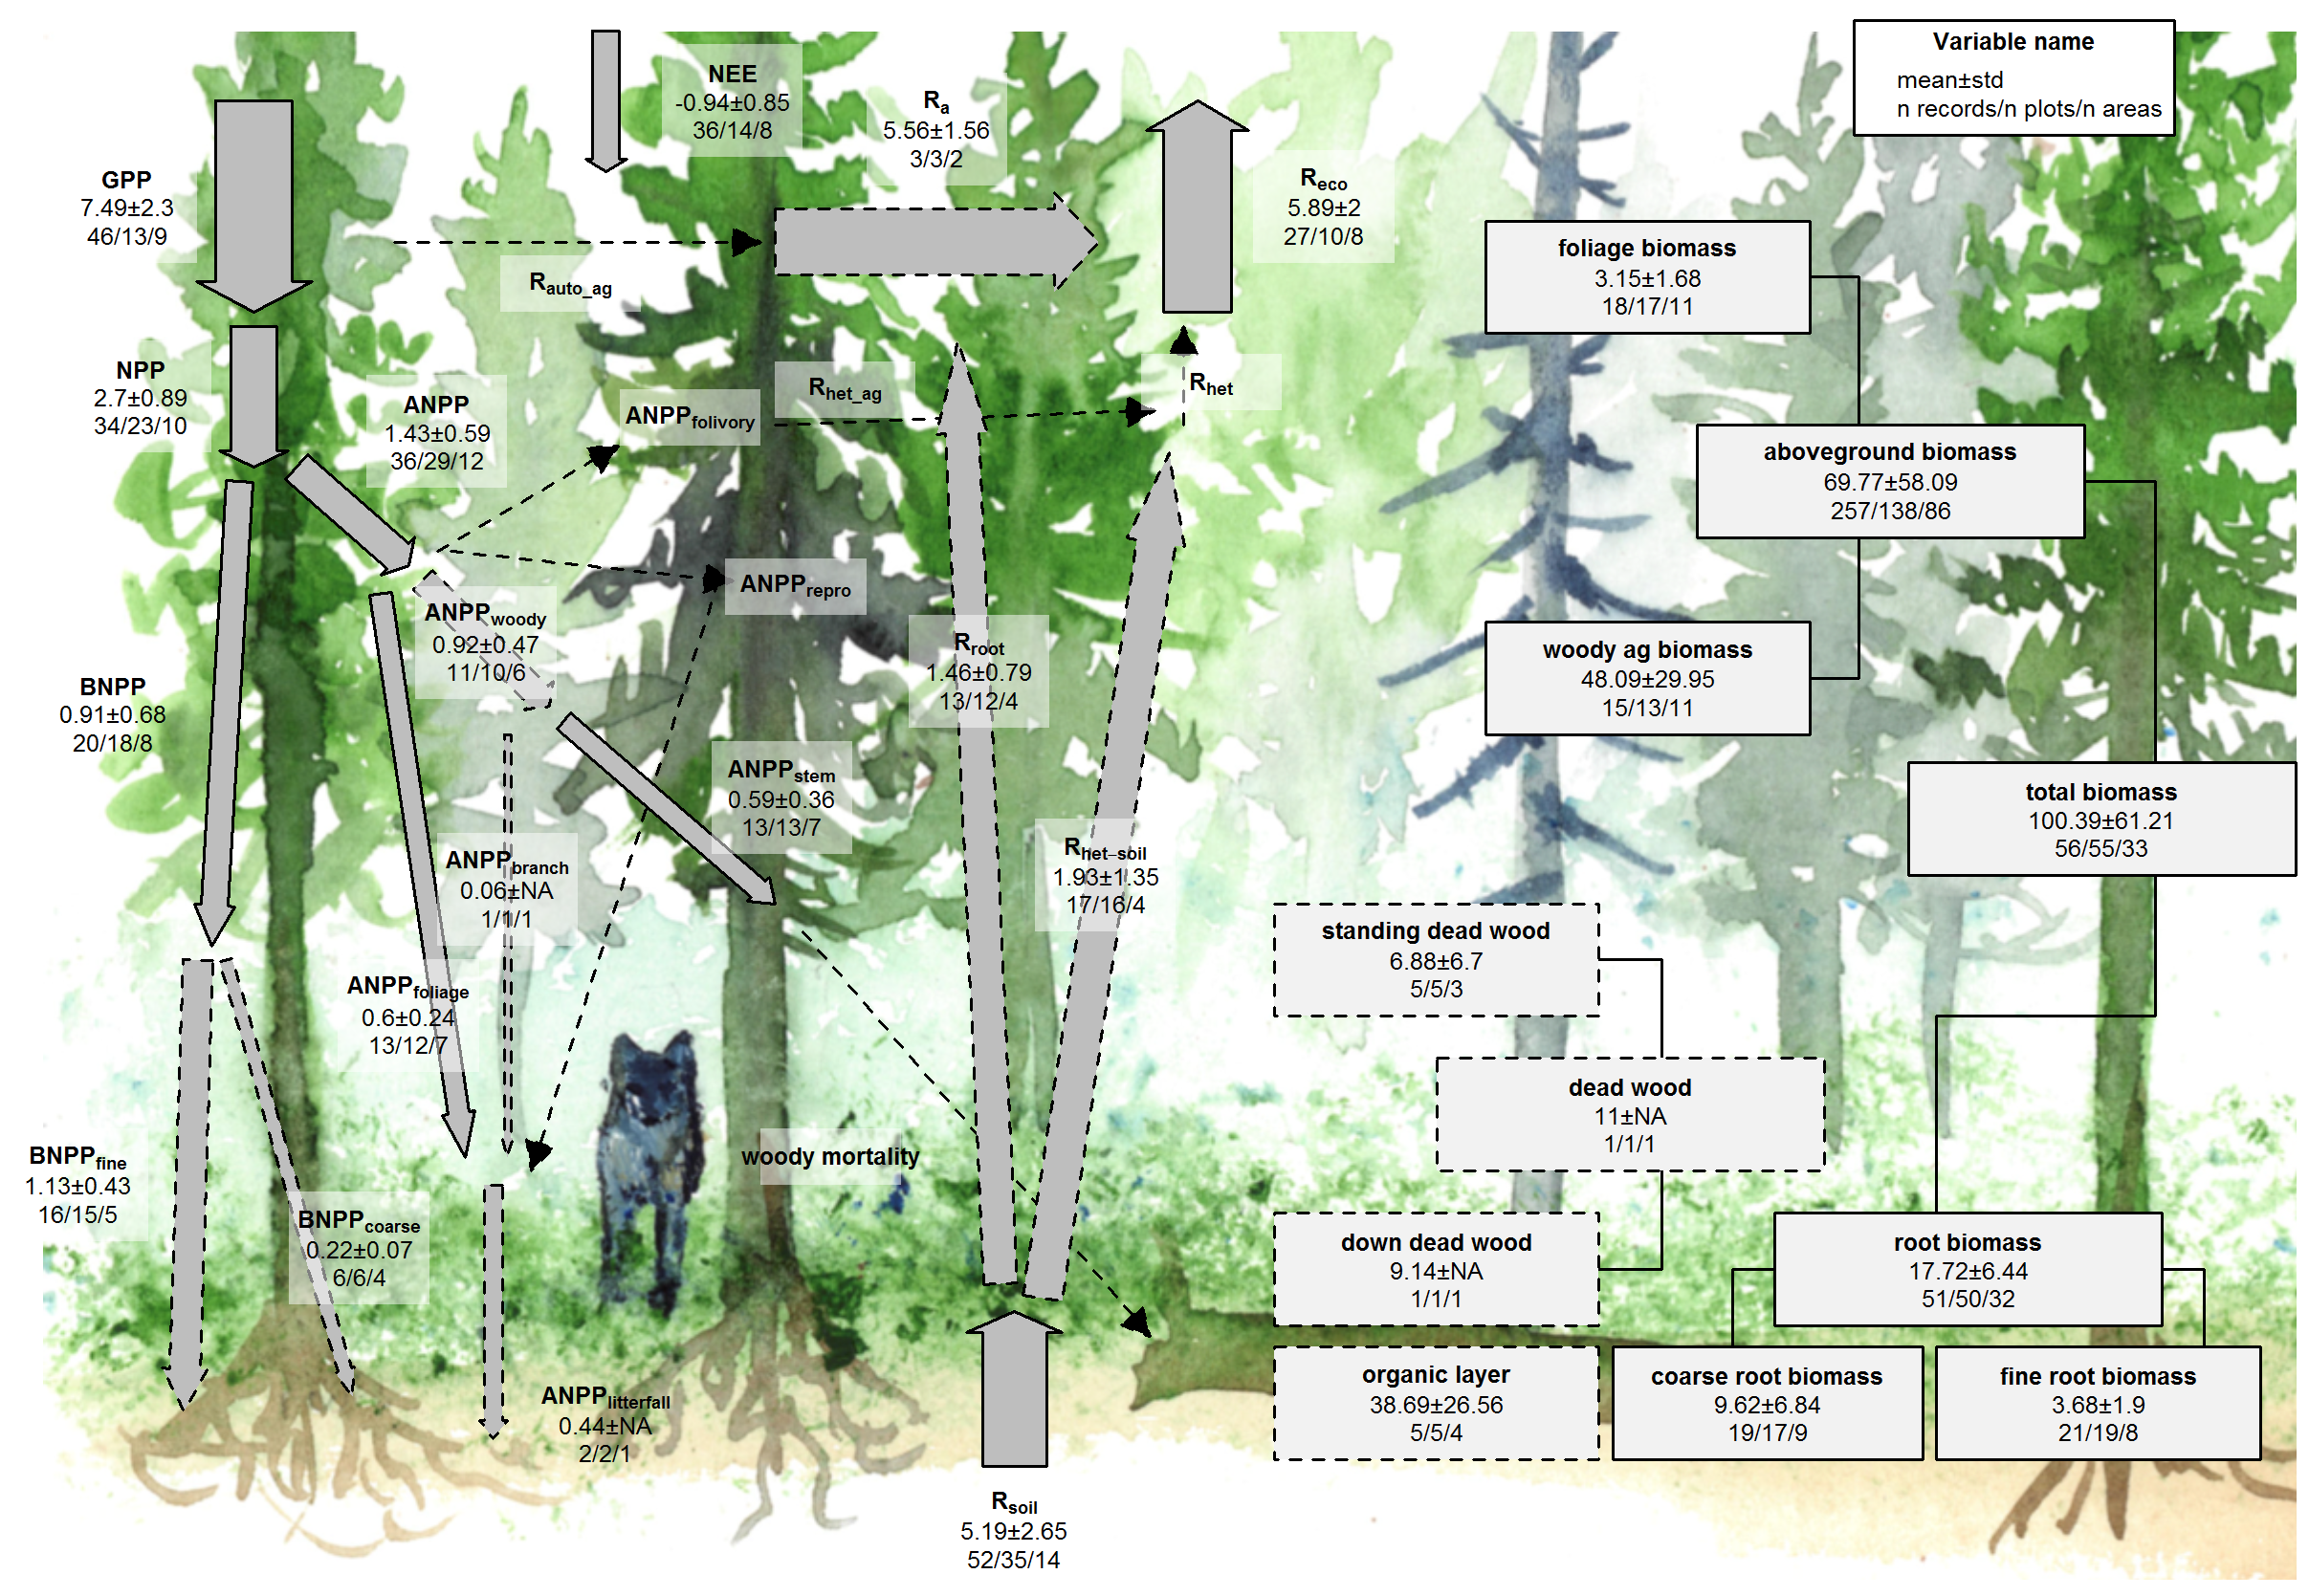
\includegraphics[width=1\linewidth]{/Users/kteixeira/Dropbox (Smithsonian)/GitHub/ForC-db/ForC/figures/C_cycle_diagrams/Diagrams/Boreal conifer MATURE} 

}

\caption{Figure 5 | C cycle diagram for mature boreal conifer forests. Arrows indicate fluxes (Mg C ha$^{-1}$ yr$^{-1}$); boxes indicate stocks (Mg C ha$^{-1}$), with variables as defined in Table 1. Presented are mean ± std, where geographically distinct areas are treated as the unit of replication. Dashed shape outlines indicate variables with records from <7 distinct geographic areas, and dashed arrows indicate fluxes with no data. To illustrate the magnitude of different fluxes, arrow size is proportional to the square root of corresponding flux. Asterisk after variable name indicates lack of C cycle closure.}\label{fig:unnamed-chunk-12}
\end{figure}
\end{landscape}

There were sufficient data to assess mature forest biome differences for
15 flux variables, and significant differences among biomes were
detected for 12 variables (Table 1). In all of these cases--including C
fluxes into, within, and out of the ecosystem--C fluxes were highest in
tropical forests, intermediate in temperate (broadleaf or conifer)
forests, and lowest in boreal forests (Table 1, Figs. 6, S1-S15).
Differences between tropical and boreal forests were always significant,
with temperate forests intermediate and significantly different from one
or both. Fluxes tended to be numerically greater in temperate broadleaf
than conifer forests, but the difference was never statistically
significant. This pattern held for the following variables: \(GPP\),
\(NPP\), \(ANPP\), \(ANPP_{stem}\),\(ANPP_{branch}\),
\(ANPP_{foliage}\), \(BNPP\), \(R_{eco}\), \(R_{root}\), \(R_{soil}\),
and \(R_{het-soil}\). For two of the variables without significant
differences among biomes (\(ANPP_{litterfall}\) and \(BNPP_{fine}\);
Figs. S8 and S11, respectively), the same general trends applied but
were not statistically significant. Another exception was for
\(BNPP_{root-coarse}\), where all records came from high-biomass forests
in the US Pacific Northwest, resulting in marginally higher values for
the temperate conifer biome (Table 1, Fig. S10; differences significant
in mixed effects model but not in post-hoc pairwise comparison).

The most notable exception to the pattern of decreasing flux from
tropical to boreal biomes was \(NEP\), with no significant differences
across biomes but with the largest average in temperate broadleaf
forests, followed by tropical, boreal, and temperate conifer forests
(Figs. 5,S1).

\begin{figure}[H]

{\centering \includegraphics[width=1\linewidth]{/Users/kteixeira/Dropbox (Smithsonian)/GitHub/ForC-db/ForC/figures/age_trends/for_ERL_review/Flux_age_trends} 

}

\caption{Figure 6 | Age trends and biome differences in some of the major C fluxes: (a) $GPP$, (b) $NPP$, (c) $ANPP$, (d) $R_{soil}$, (e) $R_{eco}$, and (f) $NEP$. Map shows data sources ($x$ and $o$ indicate young and mature stands, respectively). In each panel, the left scatterplot shows age trends in forests up to 100 years old, as characterized by a linear mixed effects model with fixed effects of age and biome. The fitted line indicates the effect of age on flux (solid lines: significant at p<0.05, dashed lines: non-significant), and non-parallel lines indicate a significant age x biome interaction. The boxplot illustrates distribution across mature forests, with different letters indicating significant differences between biomes. Data from biomes that did not meet the sample size criteria (see Methods) are plotted, but lack regression lines (young forests) or test of differences across biomes (mature forests). Individual figures for each flux with sufficient data are given in the Supplement (Figs. S1-S15).}\label{fig:unnamed-chunk-13}
\end{figure}

There were sufficient data to assess mature forest biome differences for
nine stock variables, and significant differences among biomes were
detected for five variables (\(B_{tot}\), \(B_{ag}\), \(B_{ag-wood}\),
\(B_{foliage}\), \(B_{root-coarse}\); Table 1). C stocks had less
consistent patterns across biomes (Figs. 7, S16-S26). For \(B_{tot}\)
and \(B_{ag}\), tropical broadleaf forests had the highest biomass and
boreal forests the lowest, with temperate broadleaf and needleleaf
(\(B_{ag}\) only) intermediate. For three variables that had been
disproportionately sampled in the high-biomass forests of the US Pacific
Northwest (\(B_{ag-wood}\), \(B_{foliage}\), and \(B_{root-coarse}\)),
temperate conifer forests had significantly higher stocks than the other
biomes, which were not significantly different from one another.

\begin{figure}[H]

{\centering \includegraphics[width=1\linewidth]{/Users/kteixeira/Dropbox (Smithsonian)/GitHub/ForC-db/ForC/figures/age_trends/for_ERL_review/Stock_age_trends} 

}

\caption{Figure 7 | Age trends and biome differences in some of the major forest C stocks: (a) aboveground biomass, (b) foliage, (c) fine roots, (d) dead wood. Map shows data sources ($x$ and $o$ indicate young and mature stands, respectively). In each panel, the left scatterplot  shows age trends in forests up to 100 years old, as characterized by a linear mixed effects model with fixed effects of age and biome. The fitted line indicates the effect of age on flux (solid lines: significant at p<0.05, dashed lines: non-significant), and non-parallel lines indicate a significant age x biome interaction. The boxplot illustrates distribution across mature forests, with different letters indicating signifant differences between biomes. Data from biomes that did not meet the sample size criteria (see Methods) are plotted, but lack regression lines (young forests) or test of differences across biomes (mature forests). Individual figures for each stock with sufficient data are given in the Supplement (Figs. S16-S26).}\label{fig:unnamed-chunk-14}
\end{figure}

\hypertarget{c-cycling-in-young-forests}{%
\subsubsection{C cycling in young
forests}\label{c-cycling-in-young-forests}}

Average C cycles for forests \textless100 years old are presented in
Figures 8-11. Both C stocks and fluxes commonly increased significantly
with stand age (Tables 1, S2, Figs. 6-11, S1-S26; detailed below).

\emph{ForC} contained 16 C flux variables with sufficient data for
analyses of age trends in young forests (see Methods) (Figs. 6, S1-S15).
Of these, ten increased significantly with age: \(NEP\), \(GPP\),
\(ANPP\), \(ANPP_{woody}\), \(ANPP_{foliage}\), \(ANPP_{litterfal}\),
\(BNPP\), \(BNPP_{fine}\), \(R_{eco}\), and \(R_{root}\). The remaining
six--\(NPP\), \(ANPP_{stem}\), \(ANPP_{branch}\), \(BNPP_{coarse}\),
\(R_{soil-het}\), and \(R_{soil-het}\)-\/--displayed no significant
relationship to stand age.

Differences in C fluxes across biomes typically paralleled those
observed for mature forests, with C cycling generally most rapid in the
tropics and slowest in boreal forests. The single exception was
\(ANPP_{stem}\), for which temperate broadleaf and conifer forests had
similar flux rates than tropical forests. Notably, and in contrast to
the lack of biome differences in \(NEP\) for mature forests (Fig. 6),
the tendency for temperate forests to have greater fluxes than boreal
forests held for \(NEP\) in regrowth forests (tropical forests excluded
because of insufficient data).

In terms of C stocks, ten variables (all but standing deadwood,
\(DW_{standing}\)) had sufficient data to test for age trends (Table 1,
Figs. 7, S16-26). All of these displayed a significant overall increase
with with \(log10[stand.age]\). There were sufficient data to model age
\(\times\) biome interactions were also significant for all ten of these
C stock variables (Table S2), with living C stocks tending to accumulate
more rapidly during the early stages of forest regrowth in tropical
forests (Figs. 7, S16-S22). In the case of two non-living C stocks
(\(DW_{down}\) and \(OL\)), age \(\times\) biome interactions were such
that Specifically, \(DW_{down}\) declined with age in temperate and
boreal forests, compared to an increase with age in tropical forests
(Figs. 7, S25). Similarly, \(OL\) declined slightly with age in
temperate broadleaf forests, contrasting an increase in the other three
biomes (Figs. 7, S26).

\newpage
\begin{landscape}
\begin{figure}[H]

{\centering \includegraphics[width=1\linewidth]{/Users/kteixeira/Dropbox (Smithsonian)/GitHub/ForC-db/ForC/figures/C_cycle_diagrams/Diagrams/Tropical broadleaf YOUNG} 

}

\caption{Figure 8 | C cycle diagram for young tropical broadleaf forests. Arrows indicate fluxes (Mg C ha$^{-1}$ yr$^{-1}$); boxes indicate stocks (Mg C ha$^{-1}$), with variables as defined in Table 1. Presented are observed ranges, where geographically distinct areas are treated as the unit of replication. All units are Mg C ha$^{-1}$ yr$^{-1}$ (fluxes) or Mg C ha$^{-1}$ (stocks). Dashed shape outlines indicate variables with records from <7 distinct geographic areas, and dashed arrows indicate fluxes with no data. To illustrate the magnitude of different fluxes, arrow size is proportional to the square root of corresponding flux.}\label{fig:unnamed-chunk-15}
\end{figure}

\begin{figure}[H]

{\centering \includegraphics[width=1\linewidth]{/Users/kteixeira/Dropbox (Smithsonian)/GitHub/ForC-db/ForC/figures/C_cycle_diagrams/Diagrams/Temperate broadleaf YOUNG} 

}

\caption{Figure 9 | C cycle diagram for young temperate broadleaf forests. Arrows indicate fluxes (Mg C ha$^{-1}$ yr$^{-1}$); boxes indicate stocks (Mg C ha$^{-1}$), with variables as defined in Table 1. Presented are observed ranges, where geographically distinct areas are treated as the unit of replication. All units are Mg C ha$^{-1}$ yr$^{-1}$ (fluxes) or Mg C ha$^{-1}$ (stocks). Dashed shape outlines indicate variables with records from <7 distinct geographic areas, and dashed arrows indicate fluxes with no data. To illustrate the magnitude of different fluxes, arrow size is proportional to the square root of corresponding flux.}\label{fig:unnamed-chunk-16}
\end{figure}

\begin{figure}[H]

{\centering \includegraphics[width=1\linewidth]{/Users/kteixeira/Dropbox (Smithsonian)/GitHub/ForC-db/ForC/figures/C_cycle_diagrams/Diagrams/Temperate conifer YOUNG} 

}

\caption{Figure 10 | C cycle diagram for young temperate conifer forests. Arrows indicate fluxes (Mg C ha$^{-1}$ yr$^{-1}$); boxes indicate stocks (Mg C ha$^{-1}$), with variables as defined in Table 1. Presented are observed ranges, where geographically distinct areas are treated as the unit of replication. All units are Mg C ha$^{-1}$ yr$^{-1}$ (fluxes) or Mg C ha$^{-1}$ (stocks). Dashed shape outlines indicate variables with records from <7 distinct geographic areas, and dashed arrows indicate fluxes with no data. To illustrate the magnitude of different fluxes, arrow size is proportional to the square root of corresponding flux.}\label{fig:unnamed-chunk-17}
\end{figure}

\begin{figure}[H]

{\centering \includegraphics[width=1\linewidth]{/Users/kteixeira/Dropbox (Smithsonian)/GitHub/ForC-db/ForC/figures/C_cycle_diagrams/Diagrams/Boreal conifer YOUNG} 

}

\caption{Figure 11 | C cycle diagram for young boreal conifer forests. Arrows indicate fluxes (Mg C ha$^{-1}$ yr$^{-1}$); boxes indicate stocks (Mg C ha$^{-1}$), with variables as defined in Table 1. Presented are observed ranges, where geographically distinct areas are treated as the unit of replication. All units are Mg C ha$^{-1}$ yr$^{-1}$ (fluxes) or Mg C ha$^{-1}$ (stocks). Dashed shape outlines indicate variables with records from <7 distinct geographic areas, and dashed arrows indicate fluxes with no data. To illustrate the magnitude of different fluxes, arrow size is proportional to the square root of corresponding flux.}\label{fig:unnamed-chunk-18}
\end{figure}
\end{landscape}

\hypertarget{discussion}{%
\subsection{Discussion}\label{discussion}}

\emph{ForC} v3.0 provided unprecedented coverage of most major
variables, yielding an internally consistent picture of C cycling in the
world's major forest biomes. Carbon cycling rates generally increased
from boreal to tropical regions and with stand age. Specifically, the
major C fluxes were highest in tropical forests, intermediate in
temperate (broadleaf or conifer) forests, and lowest in boreal forests
-- a pattern that generally held for regrowth as well as mature forests
(Figs. 6-7). In contrast to C fluxes, there was little directional
variation in mature forest C stocks across biomes (Figs. 2-5, 7). The
majority of flux variables, together with most live biomass pools,
increased significantly with stand age (Figs. 6-11). Together, these
results indicate that, moving from cold to tropical climates and from
young to old stands, there is a general acceleration of C cycling,
whereas C stocks and \(NEP\) of mature forests are correlated with a
different set of factors.

\hypertarget{c-variable-coverage-and-budget-closure}{%
\subsubsection{C variable coverage and budget
closure}\label{c-variable-coverage-and-budget-closure}}

The large number of C cycle variables covered by ForC, and the general
consistency between them, provide confidence that our overall reported
means provide accurate and useful baselines for analysis -- with the
caveats that they are unlikely to be accurate representations of C
cycling for any particular forest, and that these sample means almost
certainly do not represent true biome means (particularly for temperate
conifer forests where high-biomass stands are over-represented in
\emph{ForC}).

There are of course notable holes in the ForC variable coverage (Fig. 1)
that limit the scope of our inferences here. Notably, \emph{ForC}
currently has sparse--if any--coverage of fluxes to herbivores and
higher consumers, along with the woody mortality (\(M_{woody}\)) and
dead wood stocks (Tables 1, Figs. S23-S25). Geographically, all
variables are poorly covered in Africa and Siberia, a common problem in
the carbon-cycle community (Xu and Shang 2016, Schimel \emph{et al}
2015). \emph{ForC} does not include soil carbon, which is covered by
other efforts (e.g., Köchy \emph{et al} 2015). \emph{ForC} is not
intended to replace databases that are specialized for particular parts
of the C cycle analyses, e.g., aboveground biomass (Spawn \emph{et al}
2020), land-atmosphere fluxes (Baldocchi \emph{et al} 2001), soil
respiration (Jian \emph{et al} 2020), or the human footprint in global
forests (Magnani \emph{et al} 2007).

In this analysis, the C cycle budgets for mature forests (Figs. 2-5)
generally ``close''---that is, the sums of component variables do not
differ from the larger fluxes by more than one standard deviation. On
the one hand, this reflects the general fact that ecosystem-scale
measurements tend to close the C budget more easily and consistently
than, for example, for energy balance (Stoy \emph{et al} 2013). On the
other, however, \emph{ForC} derives data from multiple heterogeneous
sources, and standard deviations within each biome are high; as a
result, the standard for C closure is relatively loose (\emph{c.f.}
Houghton 2020). Nonetheless, the lack of closure, in the one instance
where it occurs, is probably more reflective of differences in the
representation of forest types (\emph{i.e.}, disproportionate
representation of US Pacific NW for \(B_{root-coarse}\) relative to
\(B_{root}\); Fig. 4) than of methodological accuracy. The overall high
degree of closure implies that \emph{ForC} gives a consistent picture of
C cycling within biomes. This is an important and useful test, because
it allows for consistency checks within the C cycle, for example
leveraging separate and independently-measured fluxes to constrain
errors in another (Phillips \emph{et al} 2017, Williams \emph{et al}
2014, Harmon \emph{et al} 2011), or producing internally consistent
global data products (Wang \emph{et al} 2018).

\hypertarget{c-cycling-across-biomes}{%
\subsubsection{C cycling across biomes}\label{c-cycling-across-biomes}}

Our analysis reveals that carbon cycling is most rapid in the tropics
and slowest in boreal regions, including C fluxes into (\(GPP\)), within
(e.g., \(NPP\) and its components), and out of (e.g., \(R_{soil}\),
\(R_{eco}\)) the ecosystem. For mature forests, this is consistent with
a large body of previous work demonstrating that C fluxes generally
decline with latitude (or increase with temperature) on a global scale
(e.g., Luyssaert \emph{et al} 2007, Gillman \emph{et al} 2015, Li and
Xiao 2019, Banbury Morgan \emph{et al} n.d.). The consistency with which
this occurs across numerous fluxes is not surprising, but has never been
simultaneously assessed across such a large number of variables (but see
Banbury Morgan \emph{et al} n.d. for nine autotrophic fluxes).

The notable exception to the pattern of fluxes decreasing from tropical
to boreal regions is \(NEP\) (Fig. 6f), which showed no significant
differences across biomes. Unlike the other C flux variables, \(NEP\)
does not characterize the rate at which C cycles through the ecosystem,
but is the balance between C sequestration (\(GPP\)) and respiratory
losses (\(R_{eco}\)) and represents net CO\textsubscript{2}
sequestration (or release) by the ecosystem. \(NEP\) tends to be
relatively small in mature forest stands (discussed further below),
which accumulate carbon slowly relative to younger stands, if at all
(Luyssaert \emph{et al} 2008, Amiro \emph{et al} 2010, Besnard \emph{et
al} 2018). It is therefore unsurprising that there are no pronounced
differences across biomes, suggesting that variation in \(NEP\) of
mature forests is controlled less by climate and more by other factors
including moderate disturbances (Curtis and Gough 2018) or
disequilibrium of \(R_{soil}\) relative to C inputs (e.g., in peatlands
where anoxic conditions inhibit decomposition; Wilson \emph{et al}
2016).

In contrast to the patterns observed for \(NEP\) in mature stands,
\(NEP\) of stands between 20 and 100 years of age varied across biomes,
being lowest in boreal forests, intermediate in temperate broadleaf
forests, and highest in temperate conifer forests (with insufficient
data to assess tropical forests; Figs. 6f, S1). This is consistent with
findings that live biomass accumulation rates (\emph{e.g.},
\(\Delta B_{ag}\) or \(\Delta B_{tot}\)) during early secondary
succession decrease with latitude (Figs. 7a, S16-S22; Anderson \emph{et
al} 2006, Cook-Patton \emph{et al} 2020). Note, though, that \(NEP\)
includes not only \(\Delta B_{tot}\), but also changes in \(DW_{tot}\),
\(OL\), and soil carbon, and biome differences in the accumulation rates
of these variables have not been detected, in part because these
variables do not consistently increase with stand age (Figs. 7, S23-S26,
and see discussion below; Cook-Patton \emph{et al} 2020).

For regrowth forests, little is known about cross-biome differences in
carbon fluxes, and we are not aware of any previous large-scale
comparisons of C fluxes that have been limited to regrowth forests.
Thus, this analysis was the first to examine flux trends in regrowth
forests across biomes. The observed tendency for young forest fluxes to
decrease from tropical to boreal regions paralleled patterns in mature
forests (Figs. 6, S1-S15), suggesting that regrowth forests follow
latitudinal trends in carbon cycling similar to those of mature forests
(e.g., Banbury Morgan \emph{et al} n.d.).

In contrast to C fluxes and biomass accumulation rates in regrowth
forests, stocks showed less systematic variation across biomes. For
aboveground biomass, which is the variable in \emph{ForC} with broadest
geographical representation, the modest trend of declining biomass from
tropical to boreal regions mirrors observations from spaceborne lidar
that reveal a decline in aboveground biomass (for all forests, including
secondary) with latitude across the N hemisphere (Hu \emph{et al} 2016).
The highest- biomass forests on Earth are, however, found in coastal
temperate climates of both the southern and northern hemisphere (Keith
\emph{et al} 2009, Smithwick \emph{et al} 2002, Hu \emph{et al} 2016).
Disproportionate representation of forests in one such region--the US
Pacific Northwest--inflated estimates of temperate conifer fluxes and
stocks for some variables and was responsible for all of the anomalous
results described here (e.g., lack of complete C budget closure,
anomalous trend across biomes for \(BNPP_{coarse}\)). Thus, biome
differences should always be interpreted relative to the geographic
distribution of sampling, which only rarely covers the majority of
forested area within a biome.

Whereas biomass can be remotely sensed and receives significant research
attention, far less is known about geographical variation in deadwood
and organic layer (\(OL\)) across biomes, which has proved a limitation
for C accounting efforts (Pan \emph{et al} 2011). Although these stocks
can be important--exceeding 100 Mg C ha\textsuperscript{-1} in some
stands (Figs. 7d-e, S23-S25), this study is the first to synthesize
deadwood data on a global scale (but see Cook-Patton \emph{et al} 2020
for young forests). Unfortunately, data remain too sparse for
statistical comparison across biomes (Figs. 7, S23-S25; but see below
for age trends), pointing to a need for more widespread quantification
of both standing and downed deadwood. \emph{ForC} coverage of \(OL\)
stocks is more comprehensive, revealing no significant differences
across temperate and tropical biomes, but a tendency towards higher
\(OL\) in boreal forests, consistent with the idea that slower
decomposition in colder climates results in more buildup of organic
matter (Allen \emph{et al} 2002). Further research on non-living C
stocks in the world's forests will be essential to completing the
picture.

\hypertarget{age-trends-in-c-cycling}{%
\subsubsection{Age trends in C cycling}\label{age-trends-in-c-cycling}}

Our study reveals that most C fluxes quickly increase to a plateau as
stands age (Fig. 6), consistent with current understanding of age trends
in forest C cycling (e.g., Anderson‐Teixeira \emph{et al} 2013, Amiro
\emph{et al} 2010, Magnani \emph{et al} 2007). While limited records in
very young (\emph{i.e.}, \textless5 year old) stands resulted in poor
resolution of the earliest phases of this increase for many variables
(sometimes detecting no age trend; Table 1), any autotrophic C flux
(e.g., \(GPP\), \(NPP\) and its components, \(R_auto\)) would be minimal
immediately following a stand-clearing disturbance. These would be
expected to increase rapidly with the most metabolically active
components of biomass, foliage and fine roots, which also increase
rapidly with stand age (Fig. 7). In contrast, soil heterotrophic
respiration (\(R_{het-soil}\)) and total soil respiration (\(R_{soil}\))
are expected to be non-zero following stand-clearing disturbance,
although these may decrease with a reduction of root respiration
(\(R_{soil}\) only) and C exudates or increase in response to an influx
of dead roots and litter (Ribeiro-Kumara \emph{et al} 2020, Maurer
\emph{et al} 2016, Bond-Lamberty \emph{et al} 2004). In this study, we
detect no significant age trends in either variable.

Notably, net carbon sequestration (\(NEP\)) increases with age up to the
100-yr threshold examined here, with more pronounced patterns in
temperate than boreal forests (Fig. 6f). This finding is largely
consistent with, but built from a far larger dataset than, previous
studies showing an increase in \(NEP\) across relatively young stand
ages (Pregitzer and Euskirchen 2004, Baldocchi \emph{et al} 2001,
Luyssaert \emph{et al} 2008). However, \(NEP\) has been observed to
decline from intermediate to old stands (Luyssaert \emph{et al} 2008),
and the \(NEP\) estimated by our model for 100-year-old temperate
conifer stands (\textasciitilde5 Mg C ha\textsuperscript{-1}
yr\textsuperscript{-1}) exceeds the mean of mature forests in the same
biome (0.7 Mg C ha\textsuperscript{-1} yr\textsuperscript{-1}; Fig.4). A
decrease in \(NEP\) is consistent with the observed deceleration of
biomass accumulation as stands age, although both biomass and non-living
C stocks will often continue to increase well beyond the 100-yr
threshold used here to delimit young and mature stands (Luyssaert
\emph{et al} 2008, McGarvey \emph{et al} 2014, Lichstein \emph{et al}
2009).

In terms of stocks, our study reveals consistent increases in live
biomass stocks with stand age--a pattern that is well-known and expected
(e.g., Lichstein \emph{et al} 2009, Yang \emph{et al} 2011)--and more
variable age trends in deadwood and \(OL\). The latter are particularly
sensitive to the type of disturbance, where disturbances that remove
most organic material (e.g., logging, agriculture) result in negligible
deadwood in young stands, followed by a buildup over time (tropical
stands in Fig. 7e; e.g., Vargas \emph{et al} 2008). In contrast, natural
disturbances (e.g., fire, drought) can produce large amounts of deadwood
(mostly \(DW_{standing}\)) that slowly decomposes as the stand recovers,
resulting in declines across young stand ages (e.g., temperate and
boreal stands in Fig. 7e; e.g., Carmona \emph{et al} 2002). Again,
further study and synthesis of non-living C stocks across biomes and
stand ages will be valuable to giving a more comprehensive picture.

\hypertarget{relevance-for-climate-change-prediction-and-mitigation}{%
\subsubsection{Relevance for climate change prediction and
mitigation}\label{relevance-for-climate-change-prediction-and-mitigation}}

The future of forest C cycling (Song \emph{et al} 2019) will shape
trends in atmospheric CO\textsubscript{2} and the course of climate
change (Schimel \emph{et al} 2015). Our findings, and more generally the
data contained in \emph{ForC} and summarized here, can help to meet two
major challenges.

First, improved representation of forest C cycling in models is
essential to improving predictions of the future course of climate
change, for the simple reason that by definition future projections
extend our existing observations and understanding to conditions that do
not currently exist on Earth (McDowell \emph{et al} 2018, Bonan and
Doney 2018, Gustafson \emph{et al} 2018). To ensure that models are
giving the right answers for the right reasons (Sulman \emph{et al}
2018), it is important to benchmark against multiple components of the C
cycle that are internally consistent with each other (Collier \emph{et
al} 2018, Wang \emph{et al} 2018). \emph{ForC}'s tens of thousands of
records are readily available in a standardized format, and our analyses
here indicate that their internal consistency is reasonably high.
Integration of \emph{ForC} with models will be valuable to improving the
accuracy and reliability of models.

Second, \emph{ForC} can serve as a pipeline through which information
can flow efficiently from forest researchers to decision-makers working
to implement forest conservation strategies at global, national, or
landscape scales. This is already happening: \emph{ForC} has contributed
to updating the IPCC guidelines for carbon accounting in forests (IPCC
2019, Requena Suarez \emph{et al} 2019), mapping C accumulation
potential from natural forest regrowth globally (Cook-Patton \emph{et
al} 2020), and informing ecosystem conservation priorities (Goldstein
\emph{et al} 2020).

It is also interesting to consider the complementary utility of
global-scale but spatially discontinuous databases such as ForC and
remote wall-to-wall remote sensing products. The latter provide
unparalleled insight into aboveground carbon stocks, but less constraint
on belowground stocks or carbon fluxes in general (Bond‐Lamberty
\emph{et al} 2016, Anav \emph{et al} 2015). Combining observational data
and remote observations may provide a much more comprehensive and
accurate picture of global forest C cycling, particularly when used in
formal data assimilation systems (Konings \emph{et al} 2019, Liu
\emph{et al} 2018). Biomass is the largest C stock in most forests, and
most of the emphasis has traditionally been on this variable.
Remote-sensing driven biomass estimates (e.g., Saatchi \emph{et al}
2011), calibrated based on high-quality ground-based data (Schepaschenko
\emph{et al} 2019, Chave \emph{et al} 2019), are well suited for this
task. Note, however, that factors such as stand age and disturbance
history are difficult, if possible, to detect remotely, and can only be
characterized for very recent decades (Hansen \emph{et al} 2013, Song
\emph{et al} 2018, Curtis \emph{et al} 2018). Ground-based data such as
\emph{ForC} are therefore valuable in defining age-based trajectories in
biomass, as in Cook-Patton \emph{et al} (2020), and thus constraining
variables such as carbon sink potential (Luyssaert \emph{et al} 2008).

In contrast, carbon allocation within forest ecosystems and respiration
fluxes cannot be remotely sensed. Efforts such as the Global Carbon
Project (Friedlingstein \emph{et al} 2019) and NASA's Carbon Monitoring
System (Liu \emph{et al} 2018) typically compute respiration as
residuals of all other terms (Bond‐Lamberty \emph{et al} 2016, Harmon
\emph{et al} 2011). This means that the errors on respiration outputs
are likely to be large and certainly poorly constrained, offering a
unique opportunity for databases such as ForC and SRDB (Jian \emph{et
al} 2020) to provide observational benchmarks. For example, Konings
\emph{et al} (2019) produced a unique top-down estimate of global
heterotrophic respiration that can both be compared with extant
bottom-up estimates (Bond‐Lamberty 2018) and used as an internal
consistency check on other parts of the carbon cycle (Phillips \emph{et
al} 2017).

\hypertarget{conclusions}{%
\subsubsection{Conclusions}\label{conclusions}}

As climate change accelerates, understanding and managing the carbon
dynamics of forests--notably including dynamics and fluxes that cannot
be observed by satellites--is critical to forecasting, mitigation, and
adaptation. The C data in \emph{ForC}, as summarized here, will be
valuable to these efforts. Notably, the fact that tropical forests tend
to have both the highest rates of C sequestration in young stands (Fig.
7; Cook-Patton \emph{et al} 2020), fueled by their generally high C flux
rates (Table 1; Fig. 6), and the highest mean biomass (Fig. 7; Table 1;
Hu \emph{et al} 2016, Jian \emph{et al} 2020) reinforces the concept
that conservation and restoration of these forests is a priority for
climate change mitigation, along with high-biomass old-growth temperate
stands (Grassi \emph{et al} 2017, Goldstein \emph{et al} 2020). It is
also important to note the trade-off in climate mitigation potential of
restoration of young forests, with high rates of CO\textsubscript{2}
sequestration (\(NEP\); Cook-Patton \emph{et al} 2020), versus
conservation and management of mature forests, with low \(NEP\) but high
C stocks that could not be recovered on a time scale relevant to climate
change mitigation (Goldstein \emph{et al} 2020). Generally speaking, the
conservation of mature forests will yield greater climate benefits
(Anderson-Teixeira and DeLucia 2011), but both approaches are critical
to avoiding catastrophic climate change (IPCC 2018).

\hypertarget{acknowledgements}{%
\subsection{Acknowledgements}\label{acknowledgements}}

Thanks to all researchers whose data are included in \emph{ForC} and
this analysis, to Jennifer McGarvey and Ian McGregor for help with the
database, and to Norbert Kunert for helpful discussion. Funding sources
included a Smithsonian Scholarly Studies grant to KAT and HML and a
Smithsonian Working Land and Seascapes grant to KAT.

\hypertarget{data-availability-statement}{%
\subsection{Data availability
statement}\label{data-availability-statement}}

Materials required to fully reproduce these analyses, including data, R
scripts, and image files, are archived in Zenodo (DOI: TBD{]}. Data,
scripts, and results presented here are also available through the
open-access \emph{ForC} GitHub repository
(\url{https://github.com/forc-db/ForC}), where many will be updated as
the database develops.

\hypertarget{references}{%
\subsection*{References}\label{references}}
\addcontentsline{toc}{subsection}{References}

\hypertarget{refs}{}
\begin{cslreferences}
\leavevmode\hypertarget{ref-allen_global_2002}{}%
Allen A, Brown J and Gillooly J 2002 Global biodiversity, biochemical
kinetics, and the energetic-equivalence rule \emph{SCIENCE} \textbf{297}
1545--8 Online:
\url{http://linkseeker.lanl.gov/unm?genre=article\&issn=0036-8075\&date=2002\&volume=297\&issue=5586\&spage=1545\&atitle=Global+biodiversity\%2C+biochemical+kinetics\%2C+and+the+energetic\%2Dequivalence+rule\&aulast=Allen\&auinit=AP}

\leavevmode\hypertarget{ref-amiro_ecosystem_2010}{}%
Amiro B D, Barr A G, Barr J G, Black T A, Bracho R, Brown M, Chen J,
Clark K L, Davis K J, Desai A R, Dore S, Engel V, Fuentes J D, Goldstein
A H, Goulden M L, Kolb T E, Lavigne M B, Law B E, Margolis H A, Martin
T, McCaughey J H, Misson L, Montes‐Helu M, Noormets A, Randerson J T,
Starr G and Xiao J 2010 Ecosystem carbon dioxide fluxes after
disturbance in forests of North America \emph{Journal of Geophysical
Research: Biogeosciences} \textbf{115} Online:
\url{http://agupubs.onlinelibrary.wiley.com/doi/abs/10.1029/2010JG001390}

\leavevmode\hypertarget{ref-anav_spatiotemporal_2015}{}%
Anav A, Friedlingstein P, Beer C, Ciais P, Harper A, Jones C,
Murray‐Tortarolo G, Papale D, Parazoo N C, Peylin P, Piao S, Sitch S,
Viovy N, Wiltshire A and Zhao M 2015 Spatiotemporal patterns of
terrestrial gross primary production: A review \emph{Reviews of
Geophysics} \textbf{53} 785--818 Online:
\url{http://agupubs.onlinelibrary.wiley.com/doi/abs/10.1002/2015RG000483}

\leavevmode\hypertarget{ref-andela_human-driven_2017}{}%
Andela N, Morton D C, Giglio L, Chen Y, Werf G R van der, Kasibhatla P
S, DeFries R S, Collatz G J, Hantson S, Kloster S, Bachelet D, Forrest
M, Lasslop G, Li F, Mangeon S, Melton J R, Yue C and Randerson J T 2017
A human-driven decline in global burned area \emph{Science} \textbf{356}
1356--62 Online:
\url{http://science.sciencemag.org/content/356/6345/1356}

\leavevmode\hypertarget{ref-anderson_temperature-dependence_2006}{}%
Anderson K J, Allen A P, Gillooly J F and Brown J H 2006
Temperature-dependence of biomass accumulation rates during secondary
succession \emph{Ecology Letters} \textbf{9} 673--82 Online:
\url{http://www.blackwell-synergy.com/doi/abs/10.1111/j.1461-0248.2006.00914.x}

\leavevmode\hypertarget{ref-anderson-teixeira_forc-dbgroa_2020}{}%
Anderson-Teixeira K, Herrmann V, CookPatton, Ferson A and Lister K 2020
Forc-db/GROA: Release with Cook-Patton et al. 2020, Nature. Online:
\url{https://zenodo.org/record/3983644}

\leavevmode\hypertarget{ref-anderson-teixeira_ctfs-forestgeo_2015}{}%
Anderson-Teixeira K J, Davies S J, Bennett A C, Gonzalez-Akre E B,
Muller-Landau H C, Joseph Wright S, Abu Salim K, Almeyda Zambrano A M,
Alonso A, Baltzer J L, Basset Y, Bourg N A, Broadbent E N, Brockelman W
Y, Bunyavejchewin S, Burslem D F R P, Butt N, Cao M, Cardenas D, Chuyong
G B, Clay K, Cordell S, Dattaraja H S, Deng X, Detto M, Du X, Duque A,
Erikson D L, Ewango C E N, Fischer G A, Fletcher C, Foster R B, Giardina
C P, Gilbert G S, Gunatilleke N, Gunatilleke S, Hao Z, Hargrove W W,
Hart T B, Hau B C H, He F, Hoffman F M, Howe R W, Hubbell S P,
Inman-Narahari F M, Jansen P A, Jiang M, Johnson D J, Kanzaki M, Kassim
A R, Kenfack D, Kibet S, Kinnaird M F, Korte L, Kral K, Kumar J, Larson
A J, Li Y, Li X, Liu S, Lum S K Y, Lutz J A, Ma K, Maddalena D M, Makana
J-R, Malhi Y, Marthews T, Mat Serudin R, McMahon S M, McShea W J,
Memiaghe H R, Mi X, Mizuno T, Morecroft M, Myers J A, Novotny V,
Oliveira A A de, Ong P S, Orwig D A, Ostertag R, Ouden J den, Parker G
G, Phillips R P, Sack L, Sainge M N, Sang W, Sri-ngernyuang K, Sukumar
R, Sun I-F, Sungpalee W, Suresh H S, Tan S, Thomas S C, Thomas D W,
Thompson J, Turner B L, Uriarte M, Valencia R, et al 2015
CTFS-ForestGEO: A worldwide network monitoring forests in an era of
global change \emph{Global Change Biology} \textbf{21} 528--49 Online:
\url{http://onlinelibrary.wiley.com/doi/10.1111/gcb.12712/abstract}

\leavevmode\hypertarget{ref-anderson-teixeira_greenhouse_2011}{}%
Anderson-Teixeira K J and DeLucia E H 2011 The greenhouse gas value of
ecosystems \emph{Global Change Biology} \textbf{17} 425--38 Online:
\url{http://doi.wiley.com/10.1111/j.1365-2486.2010.02220.x}

\leavevmode\hypertarget{ref-andersonteixeira_altered_2013}{}%
Anderson‐Teixeira K J, Miller A D, Mohan J E, Hudiburg T W, Duval B D
and DeLucia E H 2013 Altered dynamics of forest recovery under a
changing climate \emph{Global Change Biology} \textbf{19} 2001--21
Online: \url{http://onlinelibrary.wiley.com/doi/abs/10.1111/gcb.12194}

\leavevmode\hypertarget{ref-anderson-teixeira_forc_2018}{}%
Anderson-Teixeira K J, Wang M M H, McGarvey J C, Herrmann V, Tepley A J,
Bond-Lamberty B and LeBauer D S 2018 ForC: A global database of forest
carbon stocks and fluxes \emph{Ecology} \textbf{99} 1507--7 Online:
\url{http://doi.wiley.com/10.1002/ecy.2229}

\leavevmode\hypertarget{ref-anderson-teixeira_carbon_2016}{}%
Anderson-Teixeira K J, Wang M M H, McGarvey J C and LeBauer D S 2016
Carbon dynamics of mature and regrowth tropical forests derived from a
pantropical database (TropForC-db) \emph{Global Change Biology}
\textbf{22} 1690--709 Online:
\url{http://onlinelibrary.wiley.com/doi/10.1111/gcb.13226/abstract}

\leavevmode\hypertarget{ref-badgley_terrestrial_2019}{}%
Badgley G, Anderegg L D L, Berry J A and Field C B 2019 Terrestrial
gross primary production: Using NIRV to scale from site to globe
\emph{Global Change Biology} \textbf{25} 3731--40 Online:
\url{http://onlinelibrary.wiley.com/doi/abs/10.1111/gcb.14729}

\leavevmode\hypertarget{ref-baldocchi_fluxnet_2001}{}%
Baldocchi D, Falge E, Gu L, Olson R, Hollinger D, Running S, Anthoni P,
Bernhofer C, Davis K, Evans R, Fuentes J, Goldstein A, Katul G, Law B,
Lee X, Malhi Y, Meyers T, Munger W, Oechel W, Paw K T, Pilegaard K,
Schmid H P, Valentini R, Verma S, Vesala T, Wilson K and Wofsy S 2001
FLUXNET: A New Tool to Study the Temporal and Spatial Variability of
Ecosystem--Scale Carbon Dioxide, Water Vapor, and Energy Flux Densities
\emph{Bulletin of the American Meteorological Society} \textbf{82}
2415--34 Online:
\url{http://journals.ametsoc.org/doi/abs/10.1175/1520-0477(2001)082\%3C2415:FANTTS\%3E2.3.CO;2}

\leavevmode\hypertarget{ref-banbury_morgan_global_nodate}{}%
Banbury Morgan B, Herrmann V, Kunert N, Bond-Lamberty B, Muller-Landau H
C and Anderson-Teixeira K J Global patterns of forest autotrophic carbon
fluxes \emph{Global Change Biology}

\leavevmode\hypertarget{ref-bates_fitting_2015}{}%
Bates D, Mächler M, Bolker B and Walker S 2015 Fitting Linear
Mixed-Effects Models Using \textbf{lme4} \emph{Journal of Statistical
Software} \textbf{67} Online: \url{http://www.jstatsoft.org/v67/i01/}

\leavevmode\hypertarget{ref-besnard_quantifying_2018}{}%
Besnard S, Carvalhais N, Arain M A, Black A, Bruin S de, Buchmann N,
Cescatti A, Chen J, Clevers J G P W, Desai A R, Gough C M, Havrankova K,
Herold M, Hörtnagl L, Jung M, Knohl A, Kruijt B, Krupkova L, Law B E,
Lindroth A, Noormets A, Roupsard O, Steinbrecher R, Varlagin A, Vincke C
and Reichstein M 2018 Quantifying the effect of forest age in annual net
forest carbon balance \emph{Environmental Research Letters} \textbf{13}
124018 Online:
\url{https://iopscience.iop.org/article/10.1088/1748-9326/aaeaeb}

\leavevmode\hypertarget{ref-bonan_forests_2008}{}%
Bonan G B 2008 Forests and Climate Change: Forcings, Feedbacks, and the
Climate Benefits of Forests \emph{Science} \textbf{320} 1444--9 Online:
\url{http://www.sciencemag.org/cgi/content/abstract/320/5882/1444}

\leavevmode\hypertarget{ref-bonan_climate_2018}{}%
Bonan G B and Doney S C 2018 Climate, ecosystems, and planetary futures:
The challenge to predict life in Earth system models \emph{Science}
\textbf{359} Online:
\url{http://science.sciencemag.org/content/359/6375/eaam8328}

\leavevmode\hypertarget{ref-bonan_model_2019}{}%
Bonan G B, Lombardozzi D L, Wieder W R, Oleson K W, Lawrence D M,
Hoffman F M and Collier N 2019 Model Structure and Climate Data
Uncertainty in Historical Simulations of the Terrestrial Carbon Cycle
(1850--2014) \emph{Global Biogeochemical Cycles} \textbf{33} 1310--26
Online:
\url{https://onlinelibrary.wiley.com/doi/abs/10.1029/2019GB006175}

\leavevmode\hypertarget{ref-bondlamberty_new_2018}{}%
Bond‐Lamberty B 2018 New Techniques and Data for Understanding the
Global Soil Respiration Flux \emph{Earth's Future} \textbf{6} 1176--80
Online:
\url{http://agupubs.onlinelibrary.wiley.com/doi/abs/10.1029/2018EF000866}

\leavevmode\hypertarget{ref-bondlamberty_estimating_2016}{}%
Bond‐Lamberty B, Epron D, Harden J, Harmon M E, Hoffman F, Kumar J,
David McGuire A and Vargas R 2016 Estimating heterotrophic respiration
at large scales: Challenges, approaches, and next steps \emph{Ecosphere}
\textbf{7} Online:
\url{https://onlinelibrary.wiley.com/doi/abs/10.1002/ecs2.1380}

\leavevmode\hypertarget{ref-bond-lamberty_global_2010}{}%
Bond-Lamberty B and Thomson A 2010 A global database of soil respiration
data \emph{Biogeosciences} \textbf{7} 1915--26 Online:
\url{http://www.biogeosciences.net/7/1915/2010/}

\leavevmode\hypertarget{ref-bond-lamberty_contribution_2004}{}%
Bond-Lamberty B, Wang C and Gower S T 2004 Contribution of root
respiration to soil surface CO 2 flux in a boreal black spruce
chronosequence \emph{Tree Physiology} \textbf{24} 1387--95 Online:
\url{http://academic.oup.com/treephys/article/24/12/1387/1612153}

\leavevmode\hypertarget{ref-carmona_coarse_2002}{}%
Carmona M R, Armesto J J, Aravena J C and Pérez C A 2002 Coarse woody
debris biomass in successional and primary temperate forests in Chiloé
Island, Chile \emph{Forest Ecology and Management} \textbf{164} 265--75
Online:
\url{http://www.sciencedirect.com/science/article/pii/S0378112701006028}

\leavevmode\hypertarget{ref-cavaleri_urgent_2015}{}%
Cavaleri M A, Reed S C, Smith W K and Wood T E 2015 Urgent need for
warming experiments in tropical forests \emph{Global Change Biology}
\textbf{21} 2111--21 Online:
\url{http://onlinelibrary.wiley.com/doi/10.1111/gcb.12860/abstract}

\leavevmode\hypertarget{ref-chave_ground_2019}{}%
Chave J, Davies S J, Phillips O L, Lewis S L, Sist P, Schepaschenko D,
Armston J, Baker T R, Coomes D, Disney M, Duncanson L, Hérault B,
Labrière N, Meyer V, Réjou-Méchain M, Scipal K and Saatchi S 2019 Ground
Data are Essential for Biomass Remote Sensing Missions \emph{Surveys in
Geophysics} \textbf{40} 863--80 Online:
\url{https://doi.org/10.1007/s10712-019-09528-w}

\leavevmode\hypertarget{ref-collier_international_2018}{}%
Collier N, Hoffman F M, Lawrence D M, Keppel‐Aleks G, Koven C D, Riley W
J, Mu M and Randerson J T 2018 The International Land Model Benchmarking
(ILAMB) System: Design, Theory, and Implementation \emph{Journal of
Advances in Modeling Earth Systems} \textbf{10} 2731--54 Online:
\url{http://agupubs.onlinelibrary.wiley.com/doi/abs/10.1029/2018MS001354}

\leavevmode\hypertarget{ref-cook-patton_mapping_2020}{}%
Cook-Patton S C, Leavitt S M, Gibbs D, Harris N L, Lister K,
Anderson-Teixeira K J, Briggs R D, Chazdon R L, Crowther T W, Ellis P W,
Griscom H P, Herrmann V, Holl K D, Houghton R A, Larrosa C, Lomax G,
Lucas R, Madsen P, Malhi Y, Paquette A, Parker J D, Paul K, Routh D,
Roxburgh S, Saatchi S, Hoogen J van den, Walker W S, Wheeler C E, Wood S
A, Xu L and Griscom B W 2020 Mapping carbon accumulation potential from
global natural forest regrowth \emph{Nature} \textbf{585} 545--50
Online: \url{http://www.nature.com/articles/s41586-020-2686-x}

\leavevmode\hypertarget{ref-curtis_classifying_2018}{}%
Curtis P G, Slay C M, Harris N L, Tyukavina A and Hansen M C 2018
Classifying drivers of global forest loss \emph{Science} \textbf{361}
1108--11 Online:
\url{http://science.sciencemag.org/content/361/6407/1108}

\leavevmode\hypertarget{ref-curtis_forest_2018}{}%
Curtis P S and Gough C M 2018 Forest aging, disturbance and the carbon
cycle \emph{New Phytologist} \textbf{219} 1188--93 Online:
\url{http://nph.onlinelibrary.wiley.com/doi/abs/10.1111/nph.15227}

\leavevmode\hypertarget{ref-di_vittorio_initial_2020}{}%
Di Vittorio A V, Shi X, Bond‐Lamberty B, Calvin K and Jones A 2020
Initial Land Use/Cover Distribution Substantially Affects Global Carbon
and Local Temperature Projections in the Integrated Earth System Model
\emph{Global Biogeochemical Cycles} \textbf{34} Online:
\url{https://onlinelibrary.wiley.com/doi/abs/10.1029/2019GB006383}

\leavevmode\hypertarget{ref-fao_global_2010}{}%
FAO 2010 \emph{Global Forest Resources Assessment 2010} (Rome, Italy:
Food; Agriculture Organization of the United Nations)

\leavevmode\hypertarget{ref-friedlingstein_climatecarbon_2006}{}%
Friedlingstein P, Cox P, Betts R, Bopp L, Bloh W von, Brovkin V, Cadule
P, Doney S, Eby M, Fung I, Bala G, John J, Jones C, Joos F, Kato T,
Kawamiya M, Knorr W, Lindsay K, Matthews H D, Raddatz T, Rayner P, Reick
C, Roeckner E, Schnitzler K-G, Schnur R, Strassmann K, Weaver A J,
Yoshikawa C and Zeng N 2006 Climate--Carbon Cycle Feedback Analysis:
Results from the C4MIP Model Intercomparison \emph{Journal of Climate}
\textbf{19} 3337--53 Online:
\url{https://journals.ametsoc.org/doi/abs/10.1175/JCLI3800.1}

\leavevmode\hypertarget{ref-friedlingstein_global_2019}{}%
Friedlingstein P, Jones M W, O'Sullivan M, Andrew R M, Hauck J, Peters G
P, Peters W, Pongratz J, Sitch S, Le Quéré C, Bakker D C E, Canadell J
G, Ciais P, Jackson R B, Anthoni P, Barbero L, Bastos A, Bastrikov V,
Becker M, Bopp L, Buitenhuis E, Chandra N, Chevallier F, Chini L P,
Currie K I, Feely R A, Gehlen M, Gilfillan D, Gkritzalis T, Goll D S,
Gruber N, Gutekunst S, Harris I, Haverd V, Houghton R A, Hurtt G, Ilyina
T, Jain A K, Joetzjer E, Kaplan J O, Kato E, Klein Goldewijk K,
Korsbakken J I, Landschützer P, Lauvset S K, Lefèvre N, Lenton A,
Lienert S, Lombardozzi D, Marland G, McGuire P C, Melton J R, Metzl N,
Munro D R, Nabel J E M S, Nakaoka S-I, Neill C, Omar A M, Ono T, Peregon
A, Pierrot D, Poulter B, Rehder G, Resplandy L, Robertson E, Rödenbeck
C, Séférian R, Schwinger J, Smith N, Tans P P, Tian H, Tilbrook B,
Tubiello F N, Werf G R van der, Wiltshire A J and Zaehle S 2019 Global
Carbon Budget 2019 \emph{Earth System Science Data} \textbf{11}
1783--838 Online:
\url{https://essd.copernicus.org/articles/11/1783/2019/}

\leavevmode\hypertarget{ref-gillman_latitude_2015}{}%
Gillman L N, Wright S D, Cusens J, McBride P D, Malhi Y and Whittaker R
J 2015 Latitude, productivity and species richness \emph{Global Ecology
and Biogeography} \textbf{24} 107--17 Online:
\url{https://onlinelibrary.wiley.com/doi/abs/10.1111/geb.12245}

\leavevmode\hypertarget{ref-goldstein_protecting_2020}{}%
Goldstein A, Turner W R, Spawn S A, Anderson-Teixeira K J, Cook-Patton
S, Fargione J, Gibbs H K, Griscom B, Hewson J H, Howard J F, Ledezma J
C, Page S, Koh L P, Rockström J, Sanderman J and Hole D G 2020
Protecting irrecoverable carbon in Earth's ecosystems \emph{Nature
Climate Change} 1--9 Online:
\url{http://www.nature.com/articles/s41558-020-0738-8}

\leavevmode\hypertarget{ref-grassi_key_2017}{}%
Grassi G, House J, Dentener F, Federici S, Elzen M den and Penman J 2017
The key role of forests in meeting climate targets requires science for
credible mitigation \emph{Nature Climate Change} \textbf{7} 220--6
Online: \url{https://www.nature.com/articles/nclimate3227}

\leavevmode\hypertarget{ref-griscom_natural_2017}{}%
Griscom B W, Adams J, Ellis P W, Houghton R A, Lomax G, Miteva D A,
Schlesinger W H, Shoch D, Siikamäki J V, Smith P, Woodbury P, Zganjar C,
Blackman A, Campari J, Conant R T, Delgado C, Elias P, Gopalakrishna T,
Hamsik M R, Herrero M, Kiesecker J, Landis E, Laestadius L, Leavitt S M,
Minnemeyer S, Polasky S, Potapov P, Putz F E, Sanderman J, Silvius M,
Wollenberg E and Fargione J 2017 Natural climate solutions
\emph{Proceedings of the National Academy of Sciences} \textbf{114}
11645--50 Online:
\url{http://www.pnas.org/lookup/doi/10.1073/pnas.1710465114}

\leavevmode\hypertarget{ref-gustafson_extrapolating_2018}{}%
Gustafson E J, Kubiske M E, Miranda B R, Hoshika Y and Paoletti E 2018
Extrapolating plot-scale CO2 and ozone enrichment experimental results
to novel conditions and scales using mechanistic modeling
\emph{Ecological Processes} \textbf{7} 31 Online:
\url{https://doi.org/10.1186/s13717-018-0142-8}

\leavevmode\hypertarget{ref-hansen_high-resolution_2013}{}%
Hansen M C, Potapov P V, Moore R, Hancher M, Turubanova S A, Tyukavina
A, Thau D, Stehman S V, Goetz S J, Loveland T R, Kommareddy A, Egorov A,
Chini L, Justice C O and Townshend J R G 2013 High-Resolution Global
Maps of 21st-Century Forest Cover Change \emph{Science} \textbf{342}
850--3 Online:
\url{http://www.sciencemag.org/cgi/doi/10.1126/science.1244693}

\leavevmode\hypertarget{ref-harmon_heterotrophic_2011}{}%
Harmon M E, Bond-Lamberty B, Tang J and Vargas R 2011 Heterotrophic
respiration in disturbed forests: A review with examples from North
America \emph{Journal of Geophysical Research} \textbf{116} Online:
\url{http://doi.wiley.com/10.1029/2010JG001495}

\leavevmode\hypertarget{ref-houghton_terrestrial_2020}{}%
Houghton R A 2020 Terrestrial fluxes of carbon in GCP carbon budgets
\emph{Global Change Biology} \textbf{26} 3006--14 Online:
\url{https://onlinelibrary.wiley.com/doi/abs/10.1111/gcb.15050}

\leavevmode\hypertarget{ref-hu_mapping_2016}{}%
Hu T, Su Y, Xue B, Liu J, Zhao X, Fang J and Guo Q 2016 Mapping Global
Forest Aboveground Biomass with Spaceborne LiDAR, Optical Imagery, and
Forest Inventory Data \emph{Remote Sensing} \textbf{8} 565 Online:
\url{http://www.mdpi.com/2072-4292/8/7/565}

\leavevmode\hypertarget{ref-ipcc_2019_2019}{}%
IPCC 2019 \emph{2019 Refinement to the 2006 IPCC Guidelines for National
Greenhouse Gas Inventories} Online:
\url{https://www.ipcc.ch/report/2019-refinement-to-the-2006-ipcc-guidelines-for-national-greenhouse-gas-inventories/}

\leavevmode\hypertarget{ref-ipcc_global_2018}{}%
IPCC 2018 \emph{Global Warming of 1.5°C. An IPCC Special Report on the
impacts of global warming of 1.5°C above pre-industrial levels and
related global greenhouse gas emission pathways, in the context of
strengthening the global response to the threat of climate change,
sustainable development, and efforts to eradicate poverty
{[}Masson-Delmotte, V., P. Zhai, H.-O. Pörtner, D. Roberts, J. Skea,
P.R. Shukla, A. Pirani, W. Moufouma-Okia, C. Péan, R. Pidcock, S.
Connors, J.B.R. Matthews, Y. Chen, X. Zhou, M.I. Gomis, E. Lonnoy, T.
Maycock, M. Tignor, and T. Waterfield (eds.){]}.} Online:
\url{https://www.ipcc.ch/sr15/}

\leavevmode\hypertarget{ref-jian_restructured_2020}{}%
Jian J, Vargas R, Anderson-Teixeira K, Stell E, Herrmann V, Horn M,
Kholod N, Manzon J, Marchesi R, Paredes D and Bond-Lamberty B 2020
\emph{A restructured and updated global soil respiration database
(SRDB-V5)} (Data, Algorithms,; Models) Online:
\url{https://essd.copernicus.org/preprints/essd-2020-136/}

\leavevmode\hypertarget{ref-johnson_climate_2018}{}%
Johnson D J, Needham J, Xu C, Massoud E C, Davies S J, Anderson-Teixeira
K J, Bunyavejchewin S, Chambers J Q, Chang-Yang C-H, Chiang J-M, Chuyong
G B, Condit R, Cordell S, Fletcher C, Giardina C P, Giambelluca T W,
Gunatilleke N, Gunatilleke S, Hsieh C-F, Hubbell S, Inman-Narahari F,
Kassim A R, Katabuchi M, Kenfack D, Litton C M, Lum S, Mohamad M,
Nasardin M, Ong P S, Ostertag R, Sack L, Swenson N G, Sun I F, Tan S,
Thomas D W, Thompson J, Umaña M N, Uriarte M, Valencia R, Yap S,
Zimmerman J, McDowell N G and McMahon S M 2018 Climate sensitive
size-dependent survival in tropical trees \emph{Nature Ecology \&
Evolution} \textbf{2} 1436--42 Online:
\url{http://www.nature.com/articles/s41559-018-0626-z}

\leavevmode\hypertarget{ref-jung_exploiting_2006}{}%
Jung M, Henkel K, Herold M and Churkina G 2006 Exploiting synergies of
global land cover products for carbon cycle modeling \emph{Remote
Sensing of Environment} \textbf{101} 534--53 Online:
\url{http://www.sciencedirect.com/science/article/pii/S0034425706000514}

\leavevmode\hypertarget{ref-keith_re-evaluation_2009}{}%
Keith H, Mackey B G and Lindenmayer D B 2009 Re-evaluation of forest
biomass carbon stocks and lessons from the world's most carbon-dense
forests \emph{Proceedings of the National Academy of Sciences}
\textbf{106} 11635--40 Online:
\url{http://www.pnas.org/content/106/28/11635.abstract}

\leavevmode\hypertarget{ref-konings_global_2019}{}%
Konings A G, Bloom A A, Liu J, Parazoo N C, Schimel D S and Bowman K W
2019 Global satellite-driven estimates of heterotrophic respiration
\emph{Biogeosciences} \textbf{16} 2269--84 Online:
\url{https://bg.copernicus.org/articles/16/2269/2019/}

\leavevmode\hypertarget{ref-kochy_global_2015}{}%
Köchy M, Hiederer R and Freibauer A 2015 Global distribution of soil
organic carbon -- Part 1: Masses and frequency distributions of SOC
stocks for the tropics, permafrost regions, wetlands, and the world
\emph{SOIL} \textbf{1} 351--65 Online:
\url{https://soil.copernicus.org/articles/1/351/2015/}

\leavevmode\hypertarget{ref-krause_large_2018}{}%
Krause A, Pugh T A M, Bayer A D, Li W, Leung F, Bondeau A, Doelman J C,
Humpenöder F, Anthoni P, Bodirsky B L, Ciais P, Müller C,
Murray‐Tortarolo G, Olin S, Popp A, Sitch S, Stehfest E and Arneth A
2018 Large uncertainty in carbon uptake potential of land-based
climate-change mitigation efforts \emph{Global Change Biology}
\textbf{24} 3025--38 Online:
\url{https://onlinelibrary.wiley.com/doi/abs/10.1111/gcb.14144}

\leavevmode\hypertarget{ref-li_mapping_2019}{}%
Li X and Xiao J 2019 Mapping Photosynthesis Solely from Solar-Induced
Chlorophyll Fluorescence: A Global, Fine-Resolution Dataset of Gross
Primary Production Derived from OCO-2 \emph{Remote Sensing} \textbf{11}
2563 Online: \url{https://www.mdpi.com/2072-4292/11/21/2563}

\leavevmode\hypertarget{ref-lichstein_biomass_2009}{}%
Lichstein J W, Wirth C, Horn H S and Pacala S W 2009 Biomass
Chronosequences of United States Forests: Implications for Carbon
Storage and Forest Management \emph{Old-Growth Forests} Ecological
Studies ed C Wirth, G Gleixner and M Heimann (Springer Berlin
Heidelberg) pp 301--41 Online:
\url{http://link.springer.com/chapter/10.1007/978-3-540-92706-8_14}

\leavevmode\hypertarget{ref-liu_detecting_2018}{}%
Liu J, Bowman K, Parazoo N C, Bloom A A, Wunch D, Jiang Z, Gurney K R
and Schimel D 2018 Detecting drought impact on terrestrial biosphere
carbon fluxes over contiguous US with satellite observations
\emph{Environmental Research Letters} \textbf{13} 095003 Online:
\url{https://doi.org/10.1088\%2F1748-9326\%2Faad5ef}

\leavevmode\hypertarget{ref-lutz_global_2018}{}%
Lutz J A, Furniss T J, Johnson D J, Davies S J, Allen D, Alonso A,
Anderson‐Teixeira K J, Andrade A, Baltzer J, Becker K M L, Blomdahl E M,
Bourg N A, Bunyavejchewin S, Burslem D F R P, Cansler C A, Cao K, Cao M,
Cárdenas D, Chang L-W, Chao K-J, Chao W-C, Chiang J-M, Chu C, Chuyong G
B, Clay K, Condit R, Cordell S, Dattaraja H S, Duque A, Ewango C E N,
Fischer G A, Fletcher C, Freund J A, Giardina C, Germain S J, Gilbert G
S, Hao Z, Hart T, Hau B C H, He F, Hector A, Howe R W, Hsieh C-F, Hu
Y-H, Hubbell S P, Inman‐Narahari F M, Itoh A, Janík D, Kassim A R,
Kenfack D, Korte L, Král K, Larson A J, Li Y, Lin Y, Liu S, Lum S, Ma K,
Makana J-R, Malhi Y, McMahon S M, McShea W J, Memiaghe H R, Mi X,
Morecroft M, Musili P M, Myers J A, Novotny V, Oliveira A de, Ong P,
Orwig D A, Ostertag R, Parker G G, Patankar R, Phillips R P, Reynolds G,
Sack L, Song G-Z M, Su S-H, Sukumar R, Sun I-F, Suresh H S, Swanson M E,
Tan S, Thomas D W, Thompson J, Uriarte M, Valencia R, Vicentini A, Vrška
T, Wang X, Weiblen G D, Wolf A, Wu S-H, Xu H, Yamakura T, Yap S and
Zimmerman J K 2018 Global importance of large-diameter trees
\emph{Global Ecology and Biogeography} \textbf{27} 849--64 Online:
\url{https://onlinelibrary.wiley.com/doi/abs/10.1111/geb.12747}

\leavevmode\hypertarget{ref-luyssaert_co2_2007}{}%
Luyssaert S, Inglima I, Jung M, Richardson A D, Reichstein M, Papale D,
Piao S L, Schulze E-D, Wingate L, Matteucci G, Aragao L, Aubinet M, Beer
C, Bernhofer C, Black K G, Bonal D, Bonnefond J-M, Chambers J, Ciais P,
Cook B, Davis K J, Dolman A J, Gielen B, Goulden M, Grace J, Granier A,
Grelle A, Griffis T, Grünwald T, Guidolotti G, Hanson P J, Harding R,
Hollinger D Y, Hutyra L R, Kolari P, Kruijt B, Kutsch W, Lagergren F,
Laurila T, Law B E, Maire G L, Lindroth A, Loustau D, Malhi Y, Mateus J,
Migliavacca M, Misson L, Montagnani L, Moncrieff J, Moors E, Munger J W,
Nikinmaa E, Ollinger S V, Pita G, Rebmann C, Roupsard O, Saigusa N, Sanz
M J, Seufert G, Sierra C, Smith M-L, Tang J, Valentini R, Vesala T and
Janssens I A 2007 CO2 balance of boreal, temperate, and tropical forests
derived from a global database \emph{Global Change Biology} \textbf{13}
2509--37 Online:
\url{http://onlinelibrary.wiley.com/doi/abs/10.1111/j.1365-2486.2007.01439.x}

\leavevmode\hypertarget{ref-luyssaert_old-growth_2008}{}%
Luyssaert S, Schulze E D, Borner A, Knohl A, Hessenmoller D, Law B E,
Ciais P and Grace J 2008 Old-growth forests as global carbon sinks
\emph{Nature} \textbf{455} 213 Online:
\url{http://dx.doi.org/10.1038/nature07276\%20http://www.nature.com/nature/journal/v455/n7210/suppinfo/nature07276_S1.html}

\leavevmode\hypertarget{ref-magnani_human_2007}{}%
Magnani F, Mencuccini M, Borghetti M, Berbigier P, Berninger F, Delzon
S, Grelle A, Hari P, Jarvis P G, Kolari P, Kowalski A S, Lankreijer H,
Law B E, Lindroth A, Loustau D, Manca G, Moncrieff J B, Rayment M,
Tedeschi V, Valentini R and Grace J 2007 The human footprint in the
carbon cycle of temperate and boreal forests \emph{Nature} \textbf{447}
849--51 Online: \url{http://www.nature.com/articles/nature05847}

\leavevmode\hypertarget{ref-maurer_carbon_2016}{}%
Maurer G E, Chan A M, Trahan N A, Moore D J P and Bowling D R 2016
Carbon isotopic composition of forest soil respiration in the decade
following bark beetle and stem girdling disturbances in the Rocky
Mountains \emph{Plant, Cell \& Environment} \textbf{39} 1513--23 Online:
\url{http://onlinelibrary.wiley.com/doi/abs/10.1111/pce.12716}

\leavevmode\hypertarget{ref-mcdowell_pervasive_2020}{}%
McDowell N G, Allen C D, Anderson-Teixeira K, Aukema B H, Bond-Lamberty
B, Chini L, Clark J S, Dietze M, Grossiord C, Hanbury-Brown A, Hurtt G
C, Jackson R B, Johnson D J, Kueppers L, Lichstein J W, Ogle K, Poulter
B, Pugh T A M, Seidl R, Turner M G, Uriarte M, Walker A P and Xu C 2020
Pervasive shifts in forest dynamics in a changing world \emph{Science}
\textbf{368} Online:
\url{https://science.sciencemag.org/content/368/6494/eaaz9463}

\leavevmode\hypertarget{ref-mcdowell_predicting_2018}{}%
McDowell N G, Michaletz S T, Bennett K E, Solander K C, Xu C, Maxwell R
M and Middleton R S 2018 Predicting Chronic Climate-Driven Disturbances
and Their Mitigation \emph{Trends in Ecology \& Evolution} \textbf{33}
15--27 Online:
\url{https://www.cell.com/trends/ecology-evolution/abstract/S0169-5347(17)30261-6}

\leavevmode\hypertarget{ref-mcgarvey_carbon_2014}{}%
McGarvey J C, Thompson J R, Epstein H E and Shugart H H 2014 Carbon
storage in old-growth forests of the Mid-Atlantic: Toward better
understanding the eastern forest carbon sink \emph{Ecology} \textbf{96}
311--7 Online:
\url{http://www.esajournals.org/doi/abs/10.1890/14-1154.1}

\leavevmode\hypertarget{ref-novick_ameriflux_2018}{}%
Novick K A, Biederman J A, Desai A R, Litvak M E, Moore D J P, Scott R L
and Torn M S 2018 The AmeriFlux network: A coalition of the willing
\emph{Agricultural and Forest Meteorology} \textbf{249} 444--56 Online:
\url{http://www.sciencedirect.com/science/article/pii/S0168192317303295}

\leavevmode\hypertarget{ref-pan_large_2011}{}%
Pan Y, Birdsey R A, Fang J, Houghton R, Kauppi P E, Kurz W A, Phillips O
L, Shvidenko A, Lewis S L, Canadell J G, Ciais P, Jackson R B, Pacala S,
McGuire A D, Piao S, Rautiainen A, Sitch S and Hayes D 2011 A Large and
Persistent Carbon Sink in the World's Forests \emph{Science}
\textbf{333} 988--93 Online:
\url{http://www.sciencemag.org/content/early/2011/07/27/science.1201609.abstract}

\leavevmode\hypertarget{ref-phillips_value_2017}{}%
Phillips C L, Bond-Lamberty B, Desai A R, Lavoie M, Risk D, Tang J,
Todd-Brown K and Vargas R 2017 The value of soil respiration
measurements for interpreting and modeling terrestrial carbon cycling
\emph{Plant and Soil} \textbf{413} 1--25 Online:
\url{http://link.springer.com/10.1007/s11104-016-3084-x}

\leavevmode\hypertarget{ref-pregitzer_carbon_2004}{}%
Pregitzer K S and Euskirchen E S 2004 Carbon cycling and storage in
world forests: Biome patterns related to forest age \emph{Global Change
Biology} \textbf{10} 2052--77 Online:
\url{http://dx.doi.org/10.1111/j.1365-2486.2004.00866.x}

\leavevmode\hypertarget{ref-pugh_role_2019}{}%
Pugh T A M, Lindeskog M, Smith B, Poulter B, Arneth A, Haverd V and
Calle L 2019 Role of forest regrowth in global carbon sink dynamics
\emph{Proceedings of the National Academy of Sciences} \textbf{116}
4382--7 Online:
\url{http://www.pnas.org/lookup/doi/10.1073/pnas.1810512116}

\leavevmode\hypertarget{ref-r_core_team_r_2020}{}%
R Core Team 2020 R: A language and environment for statistical
computing. R Foundation for Statistical Computing, Vienna, Austria. URL
http://www.R-project.org/.

\leavevmode\hypertarget{ref-requena_suarez_estimating_2019}{}%
Requena Suarez D, Rozendaal D M A, Sy V D, Phillips O L, Alvarez‐Dávila
E, Anderson‐Teixeira K, Araujo‐Murakami A, Arroyo L, Baker T R, Bongers
F, Brienen R J W, Carter S, Cook‐Patton S C, Feldpausch T R, Griscom B
W, Harris N, Hérault B, Coronado E N H, Leavitt S M, Lewis S L, Marimon
B S, Mendoza A M, N'dja J K, N'Guessan A E, Poorter L, Qie L,
Rutishauser E, Sist P, Sonké B, Sullivan M J P, Vilanova E, Wang M M H,
Martius C and Herold M 2019 Estimating aboveground net biomass change
for tropical and subtropical forests: Refinement of IPCC default rates
using forest plot data \emph{Global Change Biology} \textbf{25} 3609--24
Online: \url{http://onlinelibrary.wiley.com/doi/abs/10.1111/gcb.14767}

\leavevmode\hypertarget{ref-ribeiro-kumara_how_2020}{}%
Ribeiro-Kumara C, Köster E, Aaltonen H and Köster K 2020 How do forest
fires affect soil greenhouse gas emissions in upland boreal forests? A
review \emph{Environmental Research} \textbf{184} 109328 Online:
\url{http://www.sciencedirect.com/science/article/pii/S0013935120302218}

\leavevmode\hypertarget{ref-saatchi_benchmark_2011}{}%
Saatchi S S, Harris N L, Brown S, Lefsky M, Mitchard E T A, Salas W,
Zutta B R, Buermann W, Lewis S L, Hagen S, Petrova S, White L, Silman M
and Morel A 2011 Benchmark map of forest carbon stocks in tropical
regions across three continents \emph{Proceedings of the National
Academy of Sciences} \textbf{108} 9899--904 Online:
\url{http://www.pnas.org/content/108/24/9899}

\leavevmode\hypertarget{ref-schepaschenko_forest_2019}{}%
Schepaschenko D, Chave J, Phillips O L, Lewis S L, Davies S J,
Réjou-Méchain M, Sist P, Scipal K, Perger C, Herault B, Labrière N,
Hofhansl F, Affum-Baffoe K, Aleinikov A, Alonso A, Amani C,
Araujo-Murakami A, Armston J, Arroyo L, Ascarrunz N, Azevedo C, Baker T,
Bałazy R, Bedeau C, Berry N, Bilous A M, Bilous S Y, Bissiengou P, Blanc
L, Bobkova K S, Braslavskaya T, Brienen R, Burslem D F R P, Condit R,
Cuni-Sanchez A, Danilina D, Torres D del C, Derroire G, Descroix L,
Sotta E D, d'Oliveira M V N, Dresel C, Erwin T, Evdokimenko M D, Falck
J, Feldpausch T R, Foli E G, Foster R, Fritz S, Garcia-Abril A D, Gornov
A, Gornova M, Gothard-Bassébé E, Gourlet-Fleury S, Guedes M, Hamer K C,
Susanty F H, Higuchi N, Coronado E N H, Hubau W, Hubbell S, Ilstedt U,
Ivanov V V, Kanashiro M, Karlsson A, Karminov V N, Killeen T, Koffi J-C
K, Konovalova M, Kraxner F, Krejza J, Krisnawati H, Krivobokov L V,
Kuznetsov M A, Lakyda I, Lakyda P I, Licona J C, Lucas R M, Lukina N,
Lussetti D, Malhi Y, Manzanera J A, Marimon B, Junior B H M, Martinez R
V, Martynenko O V, Matsala M, Matyashuk R K, Mazzei L, Memiaghe H,
Mendoza C, Mendoza A M, Moroziuk O V, Mukhortova L, Musa S, Nazimova D
I, Okuda T, Oliveira L C, et al 2019 The Forest Observation System,
building a global reference dataset for remote sensing of forest biomass
\emph{Scientific Data} \textbf{6} 1--11 Online:
\url{http://www.nature.com/articles/s41597-019-0196-1}

\leavevmode\hypertarget{ref-schimel_neon_2007}{}%
Schimel D, Hargrove W, Hoffman F and MacMahon J 2007 NEON: A
hierarchically designed national ecological network \emph{Frontiers in
Ecology and the Environment} \textbf{5} 59--9 Online:
\url{http://esajournals.onlinelibrary.wiley.com/doi/abs/10.1890/1540-9295\%282007\%295\%5B59\%3ANAHDNE\%5D2.0.CO\%3B2}

\leavevmode\hypertarget{ref-schimel_effect_2015}{}%
Schimel D, Stephens B B and Fisher J B 2015 Effect of increasing CO
\(_{\textrm{2}}\) on the terrestrial carbon cycle \emph{Proceedings of
the National Academy of Sciences} \textbf{112} 436--41 Online:
\url{http://www.pnas.org/lookup/doi/10.1073/pnas.1407302112}

\leavevmode\hypertarget{ref-smithwick_potential_2002}{}%
Smithwick E A H, Harmon M E, Remillard S M, Acker S A and Franklin J F
2002 Potential upper bounds of carbon stores in forests of the Pacific
Northwest \emph{Ecological Applications} \textbf{12} 1303--17 Online:
\url{http://doi.wiley.com/10.1890/1051-0761(2002)012\%5B1303:PUBOCS\%5D2.0.CO;2}

\leavevmode\hypertarget{ref-song_meta-analysis_2019}{}%
Song J, Wan S, Piao S, Knapp A K, Classen A T, Vicca S, Ciais P,
Hovenden M J, Leuzinger S, Beier C, Kardol P, Xia J, Liu Q, Ru J, Zhou
Z, Luo Y, Guo D, Adam Langley J, Zscheischler J, Dukes J S, Tang J, Chen
J, Hofmockel K S, Kueppers L M, Rustad L, Liu L, Smith M D, Templer P H,
Quinn Thomas R, Norby R J, Phillips R P, Niu S, Fatichi S, Wang Y, Shao
P, Han H, Wang D, Lei L, Wang J, Li X, Zhang Q, Li X, Su F, Liu B, Yang
F, Ma G, Li G, Liu Y, Liu Y, Yang Z, Zhang K, Miao Y, Hu M, Yan C, Zhang
A, Zhong M, Hui Y, Li Y and Zheng M 2019 A meta-analysis of 1,119
manipulative experiments on terrestrial carbon-cycling responses to
global change \emph{Nature Ecology \& Evolution} \textbf{3} 1309--20
Online: \url{http://www.nature.com/articles/s41559-019-0958-3}

\leavevmode\hypertarget{ref-song_global_2018}{}%
Song X-P, Hansen M C, Stehman S V, Potapov P V, Tyukavina A, Vermote E F
and Townshend J R 2018 Global land change from 1982 to 2016
\emph{Nature} \textbf{560} 639--43 Online:
\url{http://www.nature.com/articles/s41586-018-0411-9/}

\leavevmode\hypertarget{ref-spawn_harmonized_2020}{}%
Spawn S A, Sullivan C C, Lark T J and Gibbs H K 2020 Harmonized global
maps of above and belowground biomass carbon density in the year 2010
\emph{Scientific Data} \textbf{7} 112 Online:
\url{http://www.nature.com/articles/s41597-020-0444-4}

\leavevmode\hypertarget{ref-stoy_data-driven_2013}{}%
Stoy P C, Mauder M, Foken T, Marcolla B, Boegh E, Ibrom A, Arain M A,
Arneth A, Aurela M, Bernhofer C, Cescatti A, Dellwik E, Duce P, Gianelle
D, Gorsel E van, Kiely G, Knohl A, Margolis H, McCaughey H, Merbold L,
Montagnani L, Papale D, Reichstein M, Saunders M, Serrano-Ortiz P,
Sottocornola M, Spano D, Vaccari F and Varlagin A 2013 A data-driven
analysis of energy balance closure across FLUXNET research sites: The
role of landscape scale heterogeneity \emph{Agricultural and Forest
Meteorology} \textbf{171-172} 137--52 Online:
\url{https://linkinghub.elsevier.com/retrieve/pii/S0168192312003413}

\leavevmode\hypertarget{ref-sulman_multiple_2018}{}%
Sulman B N, Moore J A M, Abramoff R, Averill C, Kivlin S, Georgiou K,
Sridhar B, Hartman M D, Wang G, Wieder W R, Bradford M A, Luo Y, Mayes M
A, Morrison E, Riley W J, Salazar A, Schimel J P, Tang J and Classen A T
2018 Multiple models and experiments underscore large uncertainty in
soil carbon dynamics \emph{Biogeochemistry} \textbf{141} 109--23 Online:
\url{https://doi.org/10.1007/s10533-018-0509-z}

\leavevmode\hypertarget{ref-taylor_temperature_2017}{}%
Taylor P G, Cleveland C C, Wieder W R, Sullivan B W, Doughty C E,
Dobrowski S Z and Townsend A R 2017 Temperature and rainfall interact to
control carbon cycling in tropical forests ed L Liu \emph{Ecology
Letters} \textbf{20} 779--88 Online:
\url{http://doi.wiley.com/10.1111/ele.12765}

\leavevmode\hypertarget{ref-tubiello_carbon_2020}{}%
Tubiello F N, Pekkarinen A, Marklund L, Wanner N, Conchedda G, Federici
S, Rossi S and Grassi G 2020 Carbon Emissions and Removals by Forests:
New Estimates 1990\&ndash;2020 \emph{Earth System Science Data
Discussions} 1--21 Online:
\url{https://essd.copernicus.org/preprints/essd-2020-203/}

\leavevmode\hypertarget{ref-vargas_biomass_2008}{}%
Vargas R, Allen M F and Allen E B 2008 Biomass and carbon accumulation
in a fire chronosequence of a seasonally dry tropical forest
\emph{Global Change Biology} \textbf{14} 109--24 Online:
\url{http://onlinelibrary.wiley.com/doi/abs/10.1111/j.1365-2486.2007.01462.x}

\leavevmode\hypertarget{ref-wang_golum-cnp_2018}{}%
Wang Y, Ciais P, Goll D, Huang Y, Luo Y, Wang Y-P, Bloom A A, Broquet G,
Hartmann J, Peng S, Penuelas J, Piao S, Sardans J, Stocker B D, Wang R,
Zaehle S and Zechmeister-Boltenstern S 2018 GOLUM-CNP v1.0: A
data-driven modeling of carbon, nitrogen and phosphorus cycles in major
terrestrial biomes \emph{Geoscientific Model Development} \textbf{11}
3903--28 Online: \url{https://gmd.copernicus.org/articles/11/3903/2018/}

\leavevmode\hypertarget{ref-warner_spatial_2019}{}%
Warner D L, Bond‐Lamberty B, Jian J, Stell E and Vargas R 2019 Spatial
Predictions and Associated Uncertainty of Annual Soil Respiration at the
Global Scale \emph{Global Biogeochemical Cycles} \textbf{33} 1733--45
Online:
\url{https://onlinelibrary.wiley.com/doi/abs/10.1029/2019GB006264}

\leavevmode\hypertarget{ref-van_der_werf_global_2017}{}%
Werf G R van der, Randerson J T, Giglio L, Leeuwen T T van, Chen Y,
Rogers B M, Mu M, Marle M J E van, Morton D C, Collatz G J, Yokelson R J
and Kasibhatla P S 2017 Global fire emissions estimates during
1997--2016 \emph{Earth System Science Data} \textbf{9} 697--720 Online:
\url{https://essd.copernicus.org/articles/9/697/2017/}

\leavevmode\hypertarget{ref-williams_impacts_2014}{}%
Williams C A, Collatz G J, Masek J, Huang C and Goward S N 2014 Impacts
of disturbance history on forest carbon stocks and fluxes: Merging
satellite disturbance mapping with forest inventory data in a carbon
cycle model framework \emph{Remote Sensing of Environment} \textbf{151}
57--71 Online:
\url{https://linkinghub.elsevier.com/retrieve/pii/S0034425713004185}

\leavevmode\hypertarget{ref-wilson_stability_2016}{}%
Wilson R M, Hopple A M, Tfaily M M, Sebestyen S D, Schadt C W,
Pfeifer-Meister L, Medvedeff C, McFarlane K J, Kostka J E, Kolton M,
Kolka R K, Kluber L A, Keller J K, Guilderson T P, Griffiths N A,
Chanton J P, Bridgham S D and Hanson P J 2016 Stability of peatland
carbon to rising temperatures \emph{Nature Communications} \textbf{7}
13723 Online: \url{http://www.nature.com/articles/ncomms13723}

\leavevmode\hypertarget{ref-xu_contribution_2016}{}%
Xu M and Shang H 2016 Contribution of soil respiration to the global
carbon equation \emph{Journal of Plant Physiology} \textbf{203} 16--28
Online:
\url{https://linkinghub.elsevier.com/retrieve/pii/S0176161716301742}

\leavevmode\hypertarget{ref-yang_carbon_2011}{}%
Yang Y, Luo Y and Finzi A C 2011 Carbon and nitrogen dynamics during
forest stand development: A global synthesis \emph{New Phytologist}
\textbf{190} 977 Online:
\url{http://dx.doi.org/10.1111/j.1469-8137.2011.03645.x}
\end{cslreferences}

\end{document}
